\documentclass[a4paper]{article}
%% Sets page size and margins
\usepackage[a4paper,top=3cm,bottom=3cm,left=3cm,right=3cm,marginparwidth=1.75cm]{geometry}
%% Useful packages
\usepackage{amsmath,amsthm,amssymb,amsfonts}
\usepackage{graphicx}
\usepackage[colorinlistoftodos]{todonotes}
\usepackage{bbm}
\usepackage{setspace}
\usepackage{footmisc}
\usepackage{pdflscape}
\usepackage{natbib}
\usepackage{booktabs}
\usepackage{caption}
\usepackage{subcaption}
\usepackage{changepage}
\usepackage{rotating}
\usepackage{bm}

\usepackage{graphicx}
\usepackage[colorlinks=true, allcolors=blue]{hyperref}
\usepackage{url}

\renewcommand\footnotelayout{\fontsize{10}{12}\selectfont}



\interfootnotelinepenalty=10000

\newcommand{\R}{\mathbb{R}}
\newcommand{\N}{\mathbb{N}}
\newcommand{\Z}{\mathbb{Z}}
\providecommand{\C}{\mathbb{C}}

\theoremstyle{definition}
\newtheorem{defin}{Definição}

\theoremstyle{plain}
\newtheorem{theorem}[defin]{Teorema}
\newtheorem{corollary}[defin]{Corolário}

\linespread{2}
\title{The Distributional Impacts of the Electricity Transition on Pollution Exposure}

\author{Lauren Beatty\thanks{Environmental Defense Fund  \hspace{.5cm} E-mail: lbeatty1@edf.org \hspace{.5cm}Website: \href{https://lbeatty1.github.io}{https://lbeatty1.github.io}}, 
Matthias Fripp, 
Greg Schivley, 
Rangrang Zhang, 
Cameron Wade, \\ 
Oleg Lugovoy, 
Michael Roberts, 
Patricia Hildalgo}


\date{\today}

\begin{document}
\maketitle
\begin{center}
    PRELIMINARY DRAFT - PLEASE DO NOT CITE OR DISTRIBUTE
\end{center}

\begin{abstract}
    In this paper, we provide an overview of how different scenarios for the electricity transition will affect the distribution of air pollution exposure through 2050.  Currently, there are large disparities in pollution exposure across racial and socioeconomic groups resulting from historical choices about where generation facilities were cited, historical policies affecting migration and housing choices, and differences across groups in income and wealth. We use results from the Model Intercomparison Project -- a project aimed at harmonizing the inputs and comparing the outputs of multiple open-source least-cost electricity planning models.  We take those results, predict location-specific emissions of various pollutants over time, then use InMap to calculate average group-level exposures to PM2.5.  We find broad agreement across models.  Moreover, we find that deep decarbonization should lead to major improvements in air quality, and reductions in pollution exposure, along with a reduction in pollution exposure disparities.
\end{abstract}

\newpage
\section{Introduction}
Historical inequities have led to large contemporary differences in air pollution exposure across groups.  The academic and policy communities have increasingly been turning their attention towards reducing these inequities, and analyzing the equity impacts of policy.  This paper looks forward and analyzes how different plans for the U.S. electricity transition will affect group-level pollution exposure. 


There is a rich literature on the effects of electricity generation on pollution and the effects of pollution on human health and well-being. Air pollution is linked with numerous health impacts such as chronic obstructive pulmonary disease (COPD), acture lower respiratory illness (ALRI), cerebrovascular disease (CEV), ischaemic heart disease (IHD), and lung cancer, and in the United States, power generation is responsible for $31\%$ of premature mortality linked to outdoor air pollution \citep{Lelieveld2015TheScale}.

There is also a rich literature on how policies affect air pollution from power generation.  \citet{Shawhan2024PoliciesAmericans} use the  Engineering, Economic, and Environmental Electricity Simulation Tool (E4ST) to model capacity expansion and system operation combined with InMap to model how policies aimed at reducing air pollution in environmentally overburdened, disadvantaged communities (EO DACs) compare with hypothetical $\$15$ per ton carbon tax.  They find that both CO$_2$ pricing and the best performing within-DAC policies reduce mortality by approximately 1.4 to 1.5 times as much for EO DAC residences as non-EO DAC residents, a major win for reducing disparities.  However, they find that targeted policies are only slightly more effective than the carbon tax at reducing PM2.5, and that the plans are far more costly than a carbon tax.  Similarly, \citet{Goforth2022AirStrategies} use the Regional Energy Deployment System (ReEDS) along with InMAP to project how different U.S. national decarbonization strategies will affect air pollution disparities.  

This paper extends the literature by projecting air pollution impacts for a wider variety of policy scenarios, across multiple open-source least-cost electricity models.  Our results are in broad agreement with the studies of \citet{Goforth2022AirStrategies} and \citet{Shawhan2024PoliciesAmericans}.  We find that decarbonization strategies should lead to a large decrease in pollution exposure, as well as  a decline in disparities across groups in exposure.  Moreover, we find strong agreement between models.



\section{Data}

\subsection{Emissions Data}
Emissions data comes from two sources: EPA's Clean Air Markets Program Data (CAMD) and EPA's National Emissions Inventory (NEI).  The CAMD was created to track compliance with clean air programs, and thus, tracks emissions of CO$_2$, NO$_x$, and SO$_2$.  The NEI was created to track criteria pollutants, criteria precursors, and hazardous air pollutants from \textit{all} sources.  I get emissions of NH$_3$, VOC, and PM2.5 from the NEI. 

\subsection{Data for PowerGenome}
Data for the MIP was generated using PowerGenome, then modified on a model-by-model basis.  PowerGenome was designed to produce input files for the GenX capacity expansion model.  PowerGenome relies on a wide variety of data such as the National Renewable Energy Lab's (NREL) Annual Technology Baseline (ATB), the U.S. Energy Information Administration's Annual Energy Outlook, the EPA's Integrated Planning Model, and more.  For more information on PowerGenome, see the release page \citep{PowerGenome/PowerGenome:V0.6.3}.  Further details on the construction of model inputs for TEMOA, SWITCH, and USENSYS can be found in the main MIP paper at INSERT PAPER HERE.

\section{Methods}
This paper accompanies the Model Intercomparison Project. Once MIP outputs were obtained, we calculate source-specific emissions rates using empirical emissions data, downscale the results from MIP to predict location-specific aggregate emissions, then finally, run those emissions through the InMAP ISRM model. 


\subsection{Least-cost modeling}
We use four different open-source least-cost electricity planning models to solve many different scenarios. For more information on the models and scenarios, see OTHER PAPER.


\subsection{Calculating source-specific emissions rates}
\begin{enumerate}
    \item Join EIA generation data with EPA emissions data to calculate emissions rates in tons/MWh.  Many plants are in both the EPA and EIA data and can be matched directly, and have their own specific emissions rates.  For plants that cannot be matched, we take generation-weighted average emissions rates for each technology.
    \item Calculate emissions from existing plants by taking model-outputted generation and multiplying that by the plant's share of cluster capacity to get a predicted MWh.  Then multiply that by the plant's emissions rates for all five pollutants.
    \item The new fossil generation produced by these models is only natural gas or natural gas with CCS.  For new plants, we begin by allocating new capacity to retired sites.  Once the new capacity equals the retired capacity, we allocate the remaining new capacity to both existing and retired sites, weighted by capacity.  This is essentially an assumption that the spatial distribution of new generation will mirror existing and retired generation.  
\end{enumerate}


\subsection{Emissions to Exposure: InMap}
Once we've obtained predictions for plant-level emissions, we feed these emissions into the InMap Source-Receptor Matrix (ISRM).  The ISRM was developed to further simply the InMAP model.  The InMAP model was designed to compute annual-average primary and secondary PM2.5.  InMAP is not a full Eulerian chemical tranport model. Rather, InMAP uses information from chemical transport models along with some simplifying assumptions and estimated reduced-form parameters \citep{Tessum2017InMAP:Interventions}.  The InMAP ISRM was developed by running InMAP hundreds of thousands of times to calculate the average linear relationship between emissions in each source location with annual-average PM2.5 concentrations at receptor locations \citep{Goodkind2019Fine-scaleEmissions}.  The InMAP ISRM uses a variable grid with a finer scale in more population-dense areas, and a coarser definition in less dense areas, greatly reducing the size of the matrix while still maintaining it's ability to make fine-scale spatial prediction.  We plot an example of the ISRM output below in figure \ref{ISRMexample}.
\begin{figure}
    \centering
    \begin{subfigure}[b]{0.45\textwidth}
        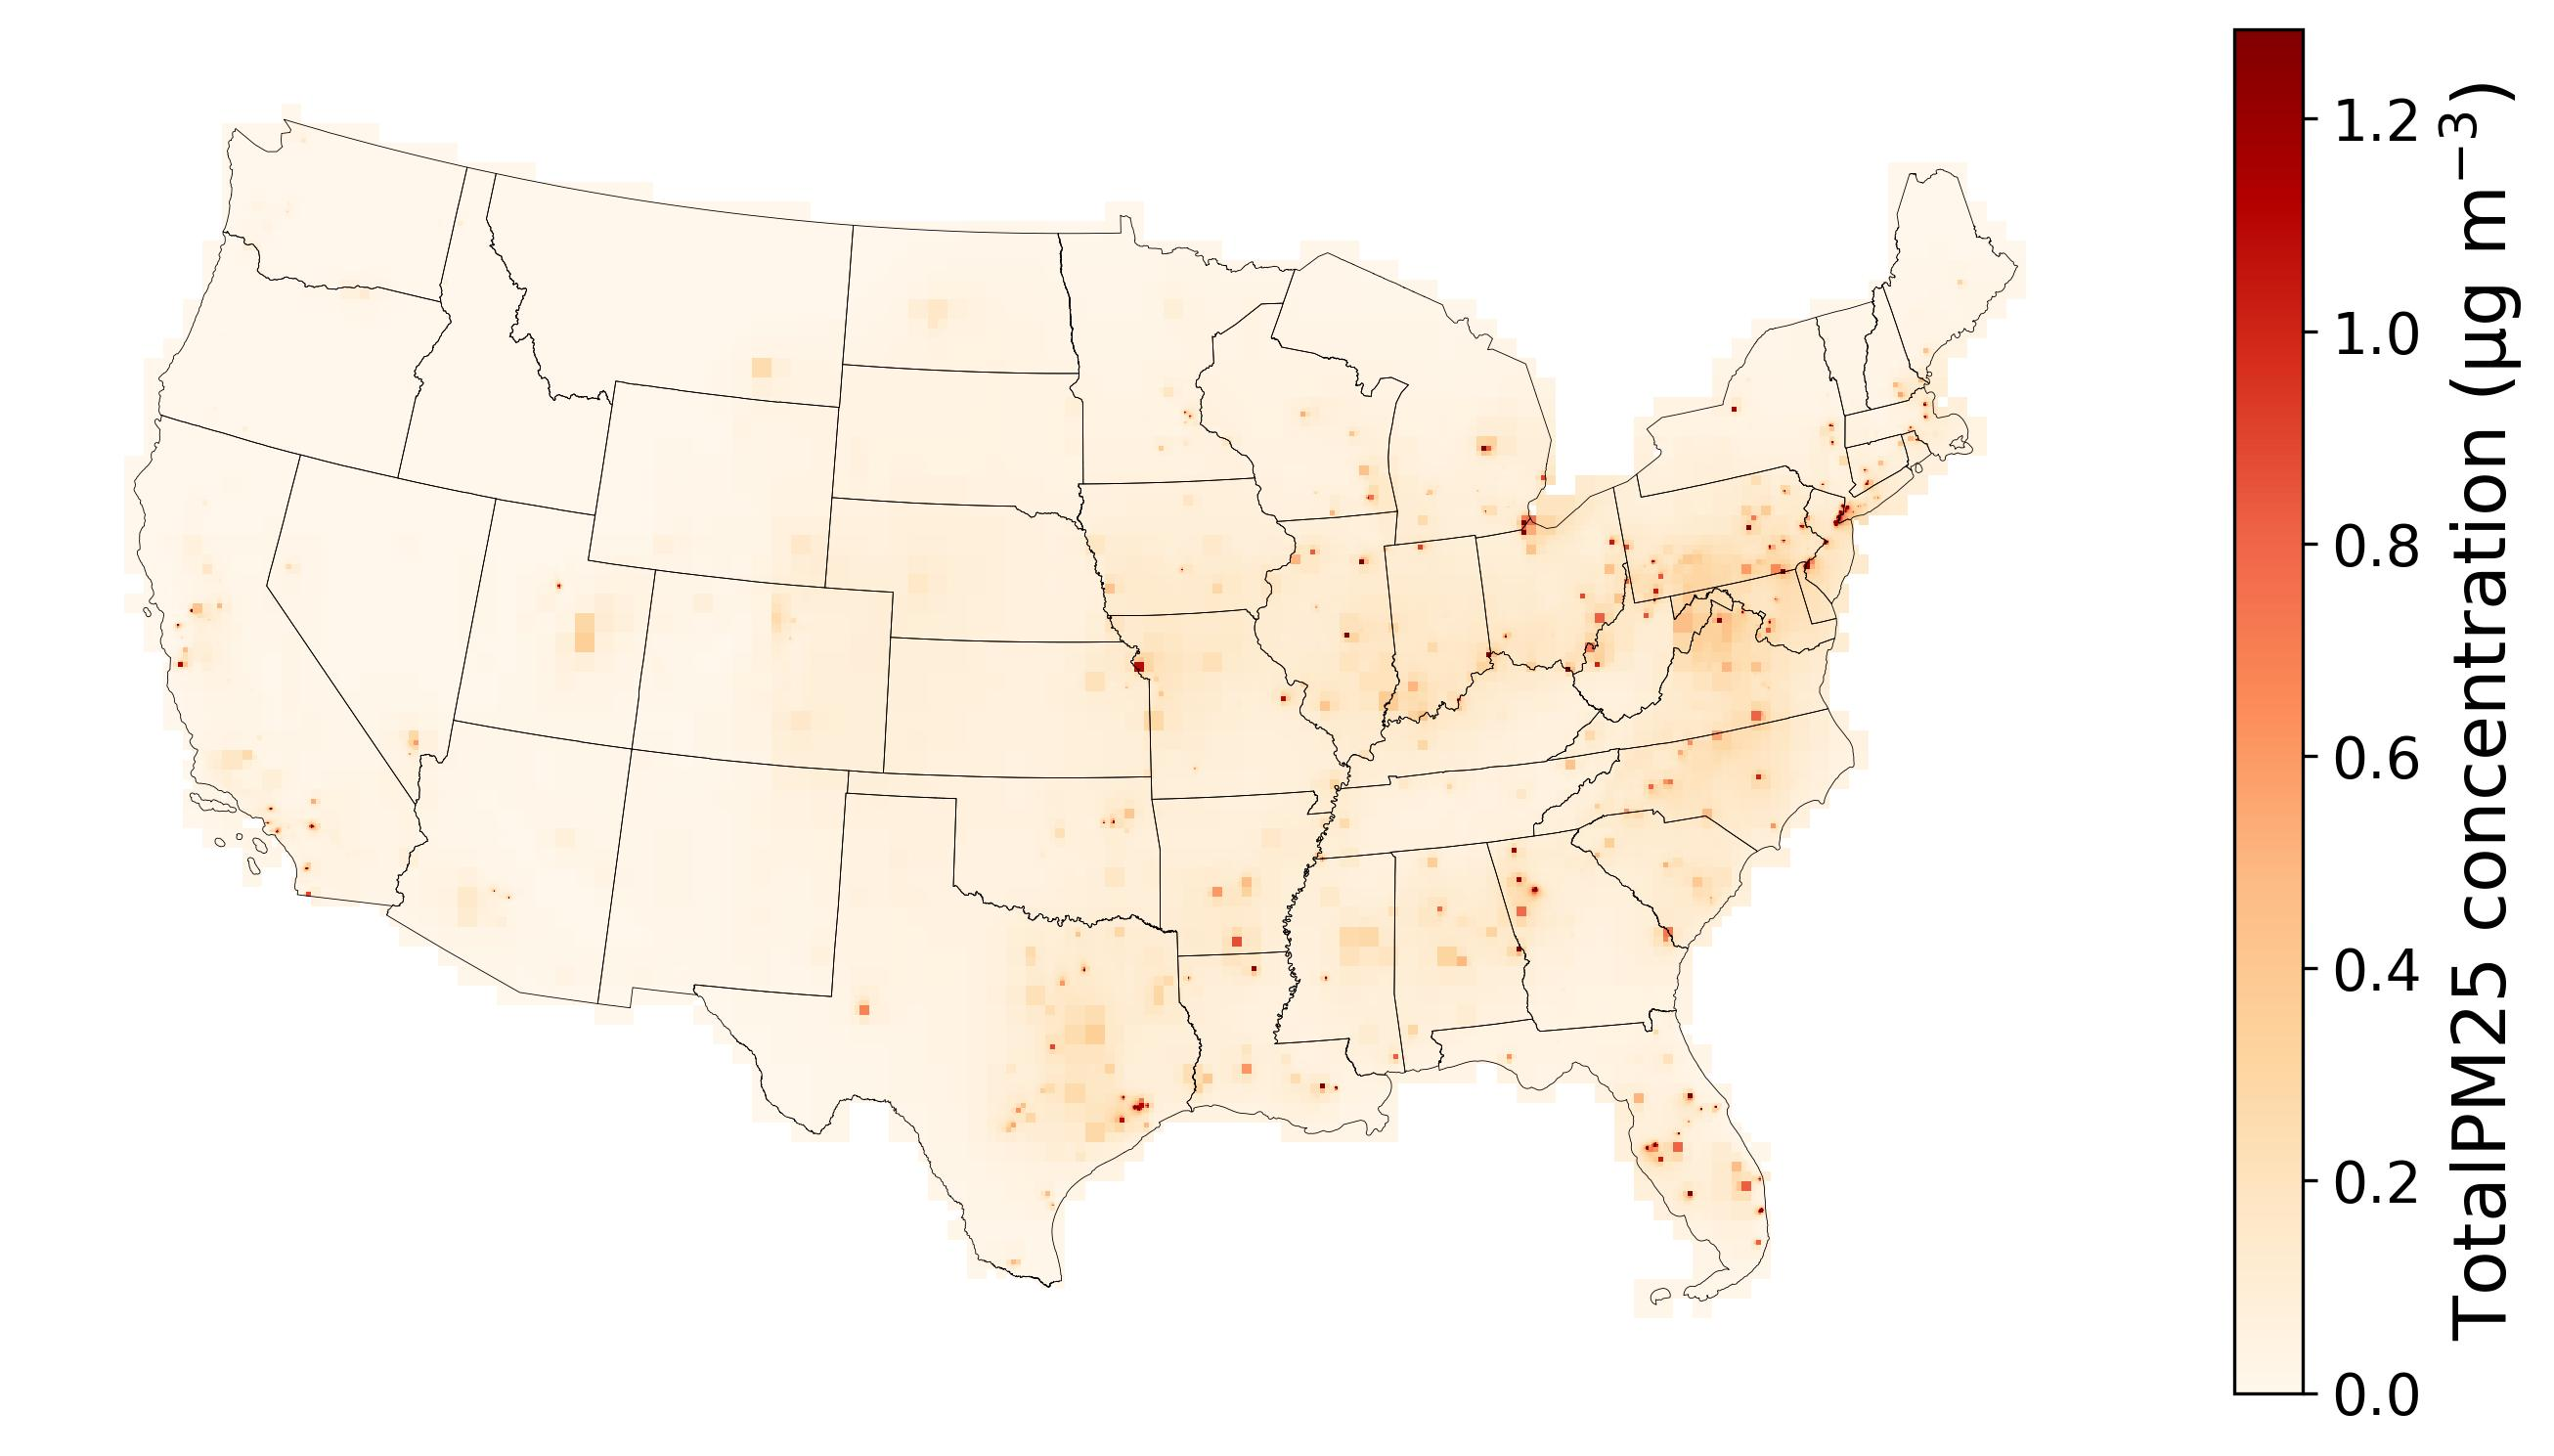
\includegraphics[width=\textwidth]{Figures/Output/full-base-200/GenX/ISRM_2027_TotalPM25_concentrationmap.jpg}
        \caption{2027}
        \label{Subfig1}
    \end{subfigure}
    \hfill
    \begin{subfigure}[b]{0.45\textwidth}
        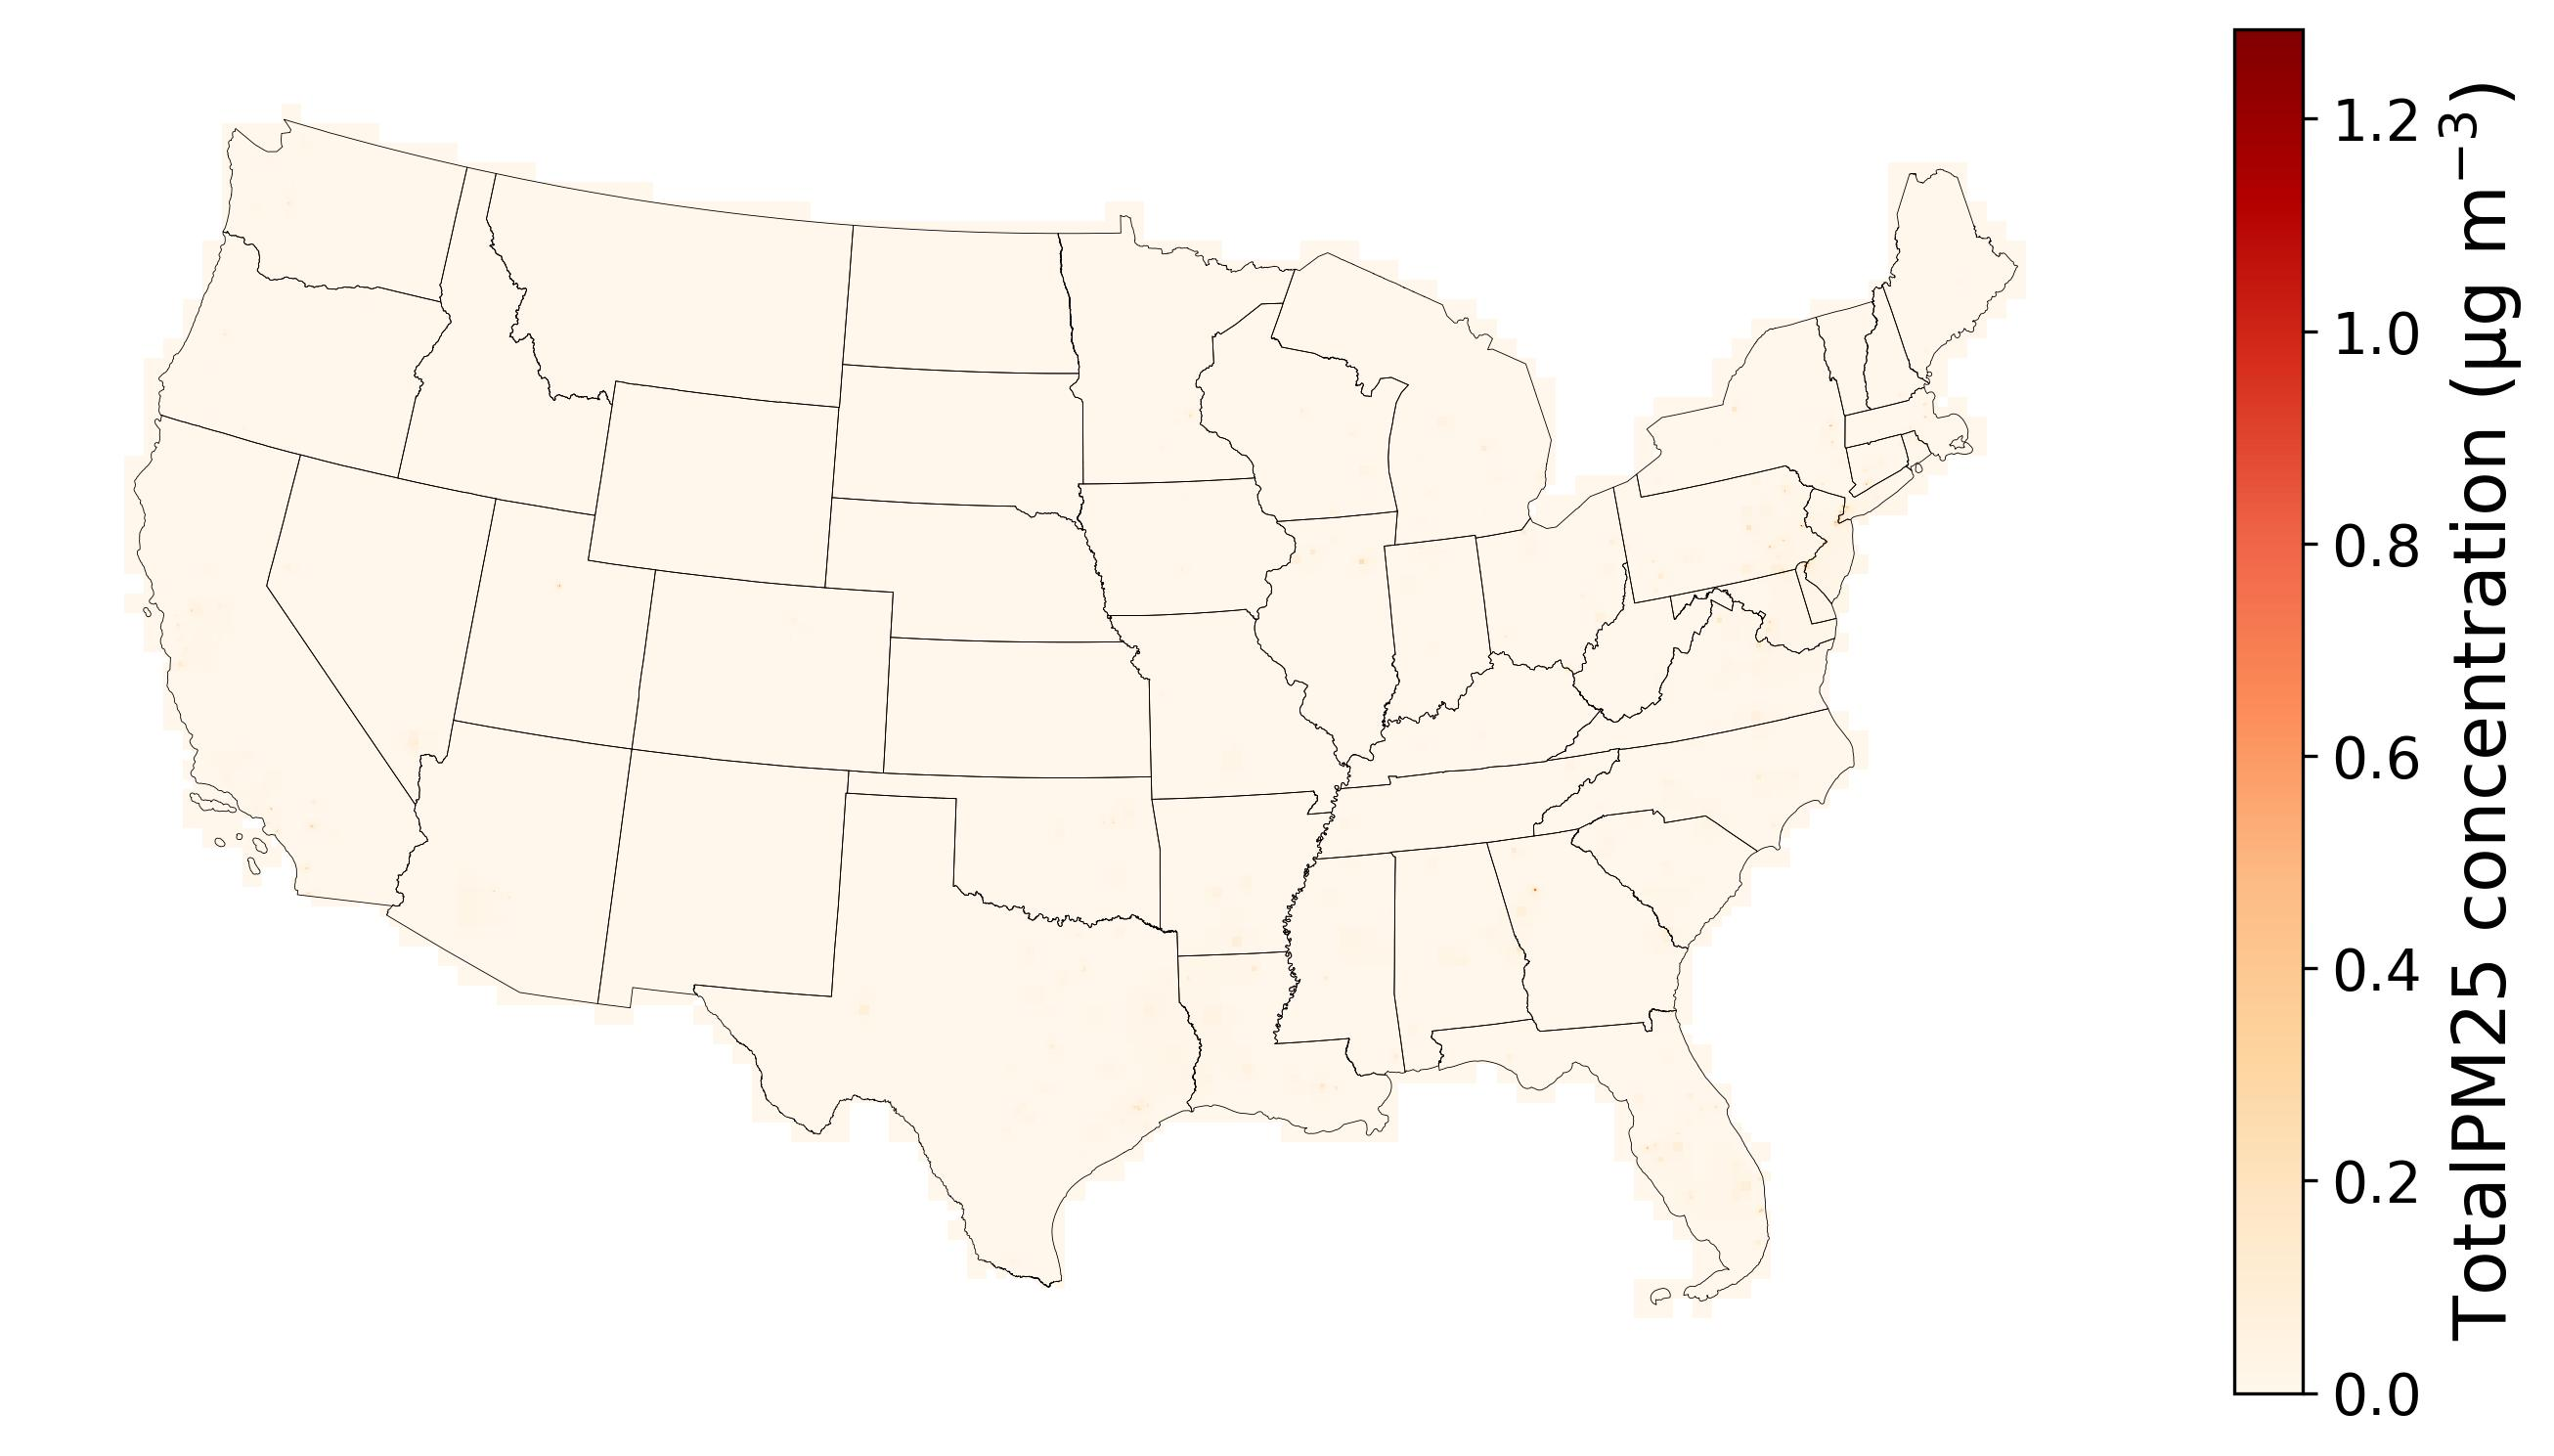
\includegraphics[width=\textwidth]{Figures/Output/full-base-200/GenX/ISRM_2050_TotalPM25_concentrationmap.jpg}
        \caption{2050}
        \label{Subfig2}
    \end{subfigure}\\
    \caption{ISRM Output for the Base Scenario in 2027 and 2050.}
\end{figure}
For each grid area, $i$, we translate concentrations into mortality using total PM2.5 predicted by INMAP in a Cox proportional hazards equation:

\begin{equation}
    Deaths_i = [\exp(\log(r)/10*PM2.5_i)-1]\times Pop_i \times \frac{Pop_y}{Pop_{2010}} \times MortalityRate_i
\end{equation}
where 
\begin{itemize}
    \item $r$ is a parameter describing how mortality rates respond to a 10$\mu g/m^3$ increase in PM2.5 concentrations.  For this paper we use 1.06, reported by \citet{Krewski2009ExtendedInstitute}.
    \item $Pop_i$ is the population of grid $i$ in 2010.
    \item $\frac{Pop_y}{Pop_{2010}}$ is the ratio between year-$y$ population and year-2010 population (what's natively in the model).  For each model period we calculate this ratio from the 2023 U.S. Census Bureau's National Population Projection Tables.  These tables have projections by race and by year, so our estimates will reflect, for example, the fact that the Hispanic and Latino population is expected to grow by 42$\%$ by 2050, while the Non-Hispanic White population is expected to decrease \citep{Bureau2023Series}.
    \item $MortalityRate_i$ is the mortality rate for grid $i$.\footnote{The mortality rate in the model is for 2005.  For simplicty, we don't replace this.  Since it remains constant over time, these projections will not account for changes in mortality rates over time.}
\end{itemize}

While the projection takes into account idiosyncratic changes across groups in population growth, it will not take into acount idiosyncratic changes across groups \textit{across space}.  In addition, our estimates will not reflect differences between groups in mortality rates, which previous work has shown may be an important driver of mortality in models \citep{Spiller2021MortalityOutcomes}.  Lastly, these projections will not take into account expected changes over time in mortality rates. Since our primary concern is differences in mortality \textit{rates} rather than aggregate mortality, we think these are reasonable assumptions and simplifications. Moreover, we primarily want our estimates to reflect changes in electricity generation, rather than population projections with wide uncertainty bands.
\section{Results: Comparison Across Models}
Our first result is that there is tight agreement across models.  This is a fairly unsurprising result in light of the results of MIP PROJECT PAPER.  The models have similar amounts of generation and capacity expansion across models, as well as similar CO$_2$ emissions and costs.  The largest difference we observe between race-specific death rates is X$\%$.

\begin{figure}
    \centering
    \begin{subfigure}[b]{0.45\textwidth}
        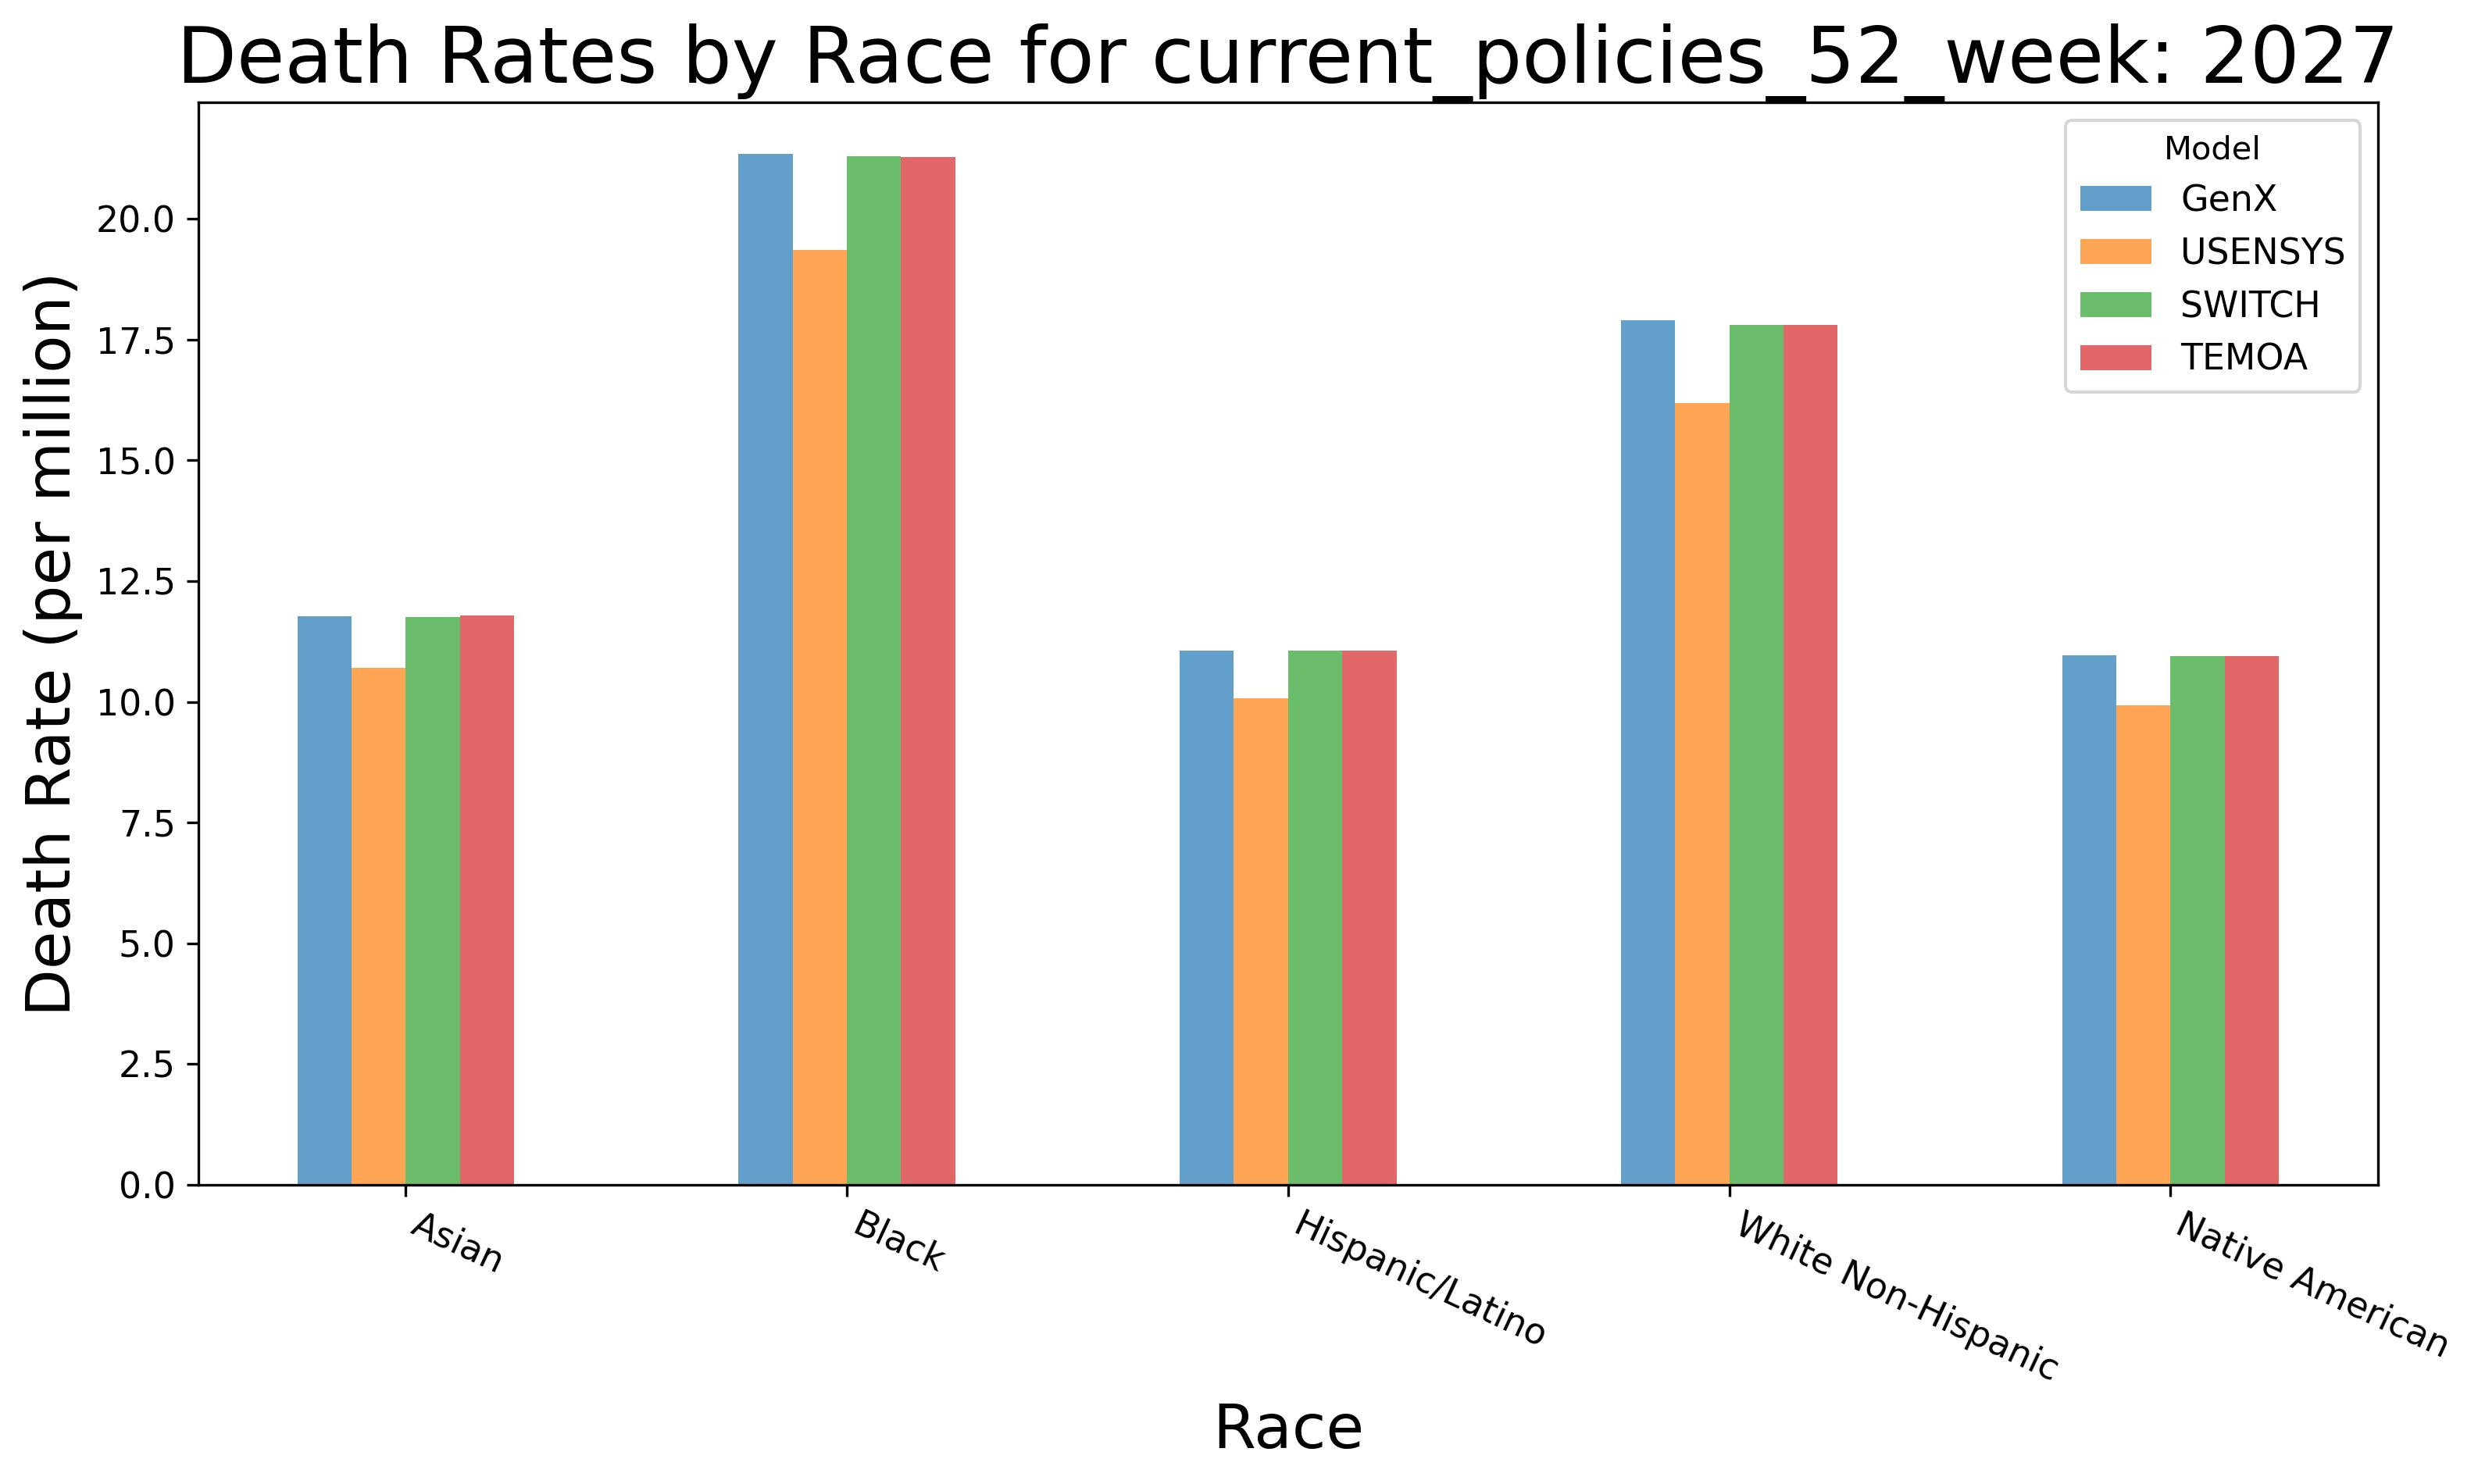
\includegraphics[width=\textwidth]{Figures/Output/DeathRate_Across_Models_current_policies_52_week_2027.png}
        \label{2027CompareModels}
    \end{subfigure}
    \hfill
    \begin{subfigure}[b]{0.45\textwidth}
        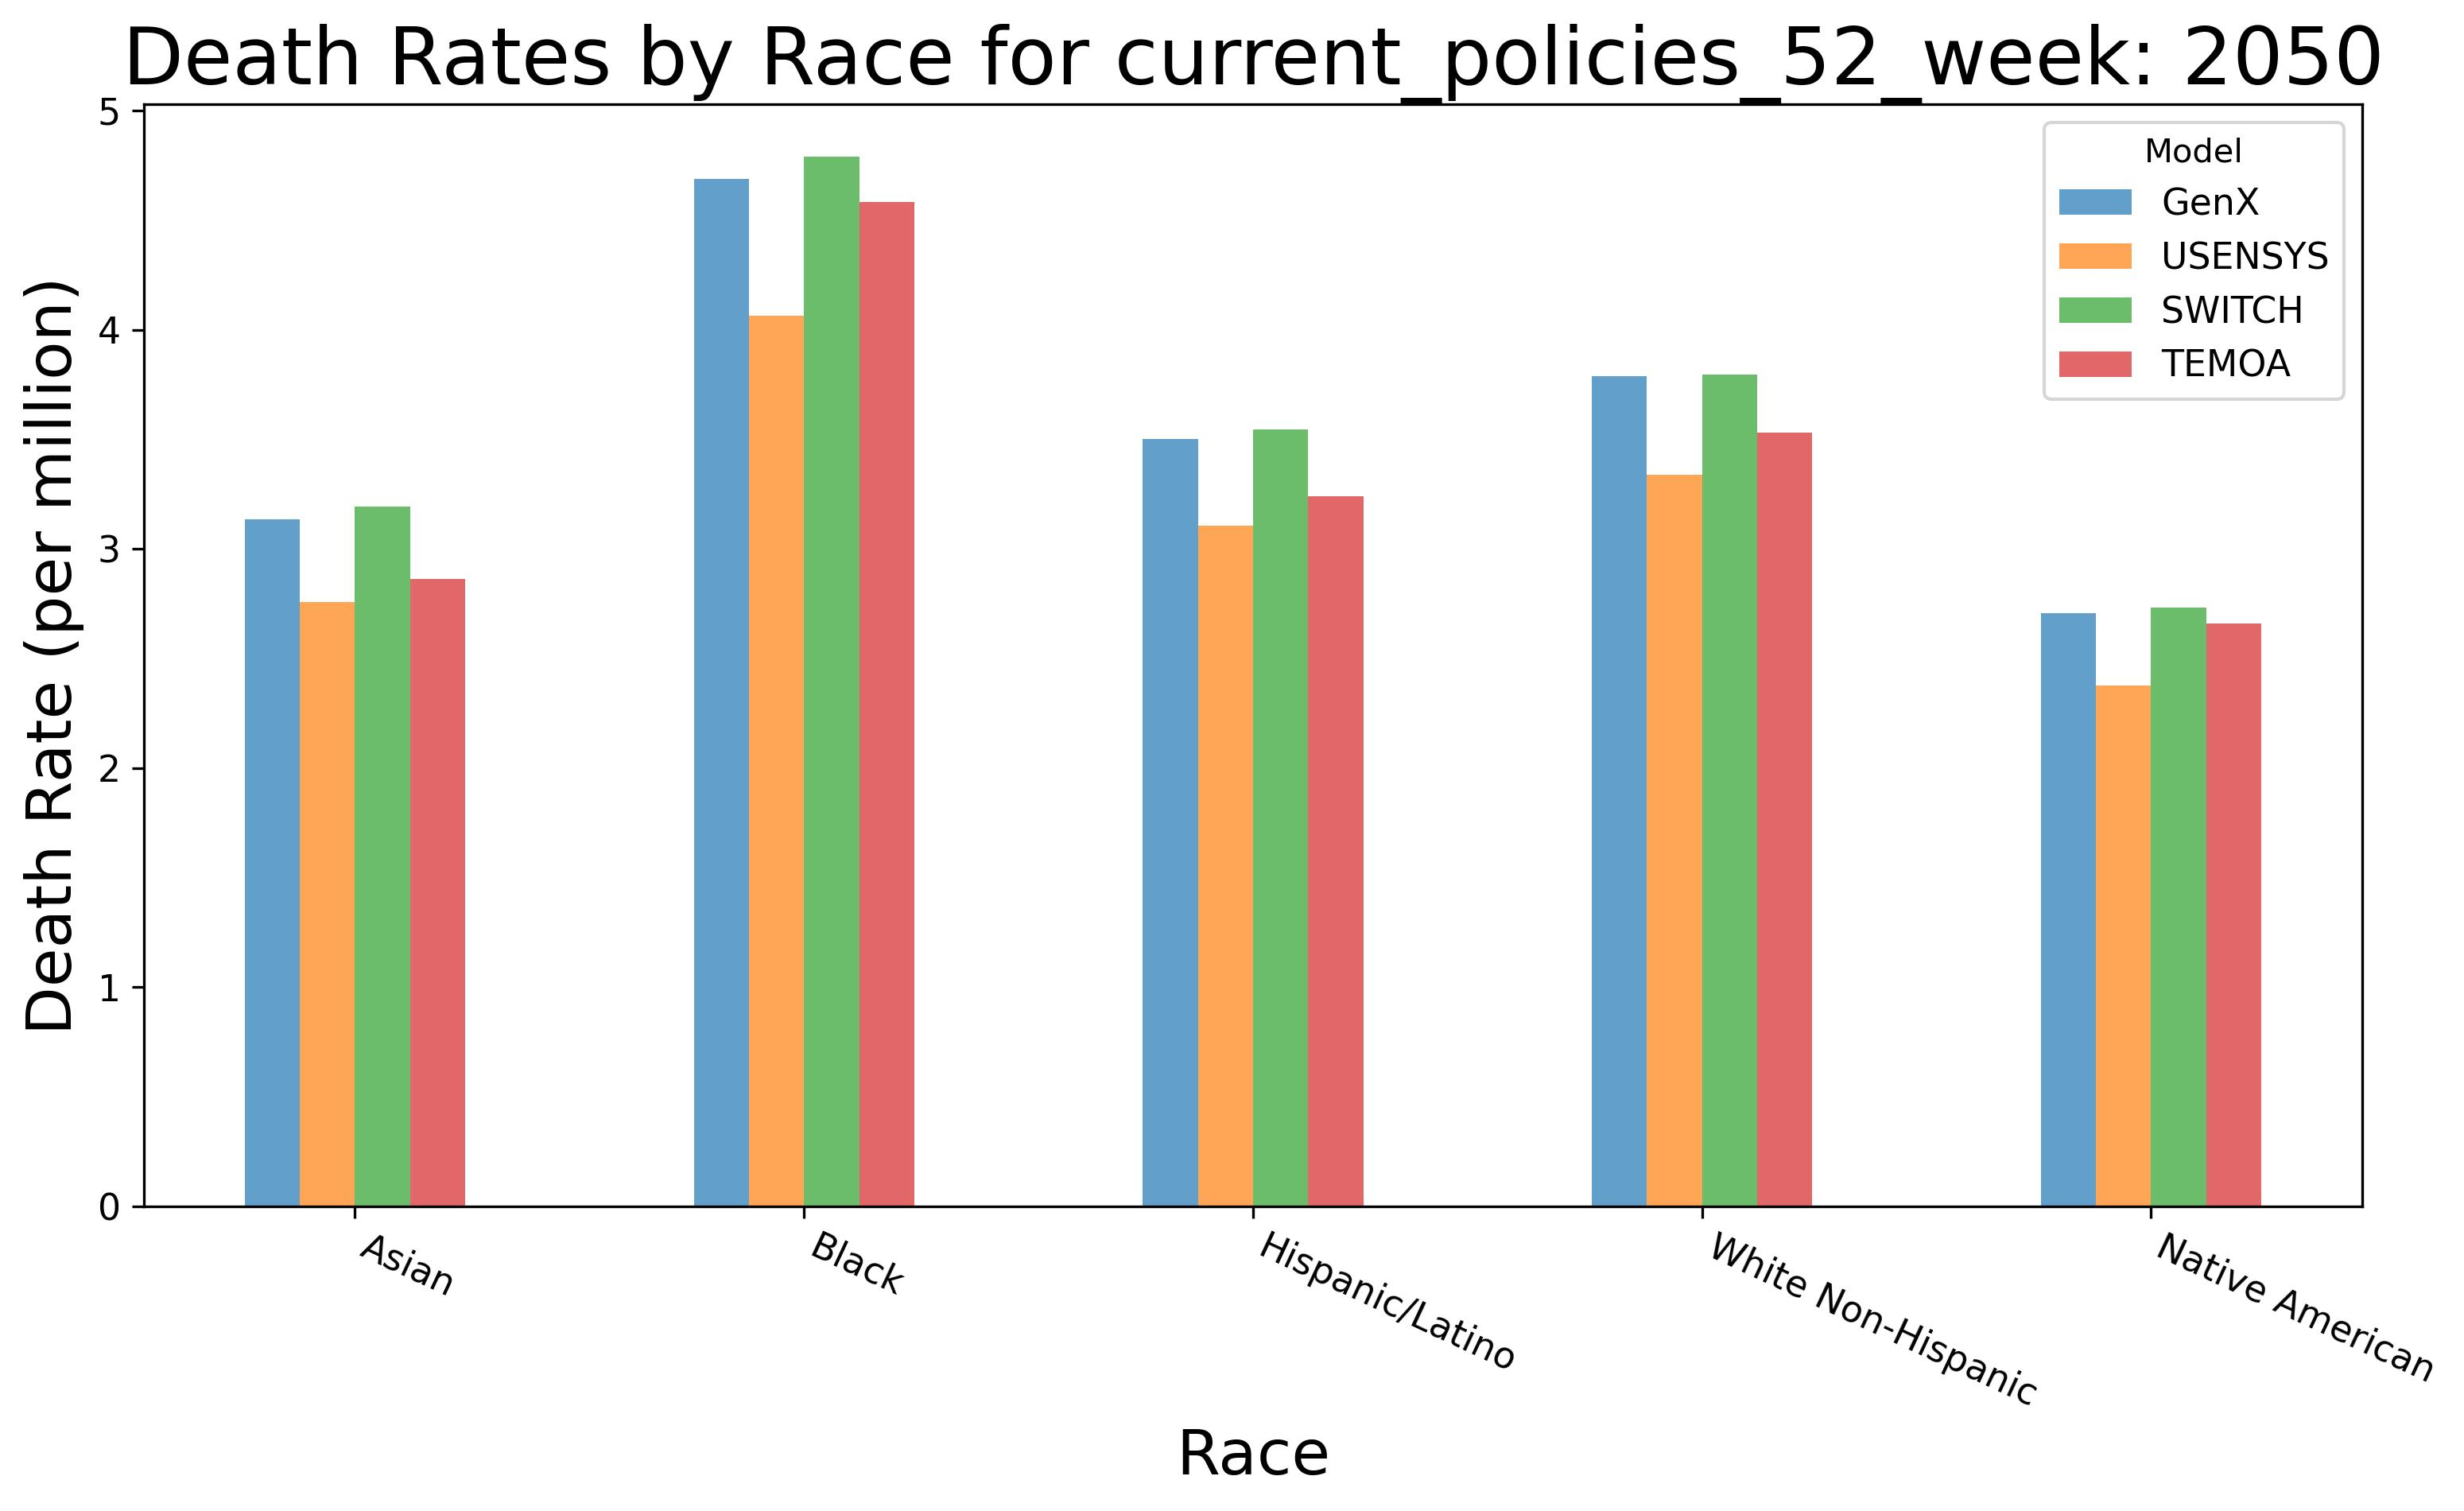
\includegraphics[width=\textwidth]{Figures/Output/DeathRate_Across_Models_current_policies_52_week_2050.png}
        \label{2050CompareModels}
    \end{subfigure}\\

    \caption{Comparison of results across models for the current policies scenario in 2027 and 2050}
    \label{Compare Scenarios}
\end{figure}


\section{Results: Comparison Across Scenarios}

Given the precise agreement between the models, we now turn our attention to comparing pollution exposure across policy scenarios.  In figure \ref{Compare Scenarios}, we plot population-weighted mean death rates by racial group by scenario for each model period.  The first thing that becomes immediately apparent is that the decarbonization scenarios reduce pollution exposure much more quickly and dramatically than the current policy scenarios.  It's also clear that there are wide disparities across racial groups, these disparities decrease in aggregate magnitudes but remain more constant in relative magnitudes over time.
\begin{figure}
    \centering
    \begin{subfigure}[b]{0.49\textwidth}
        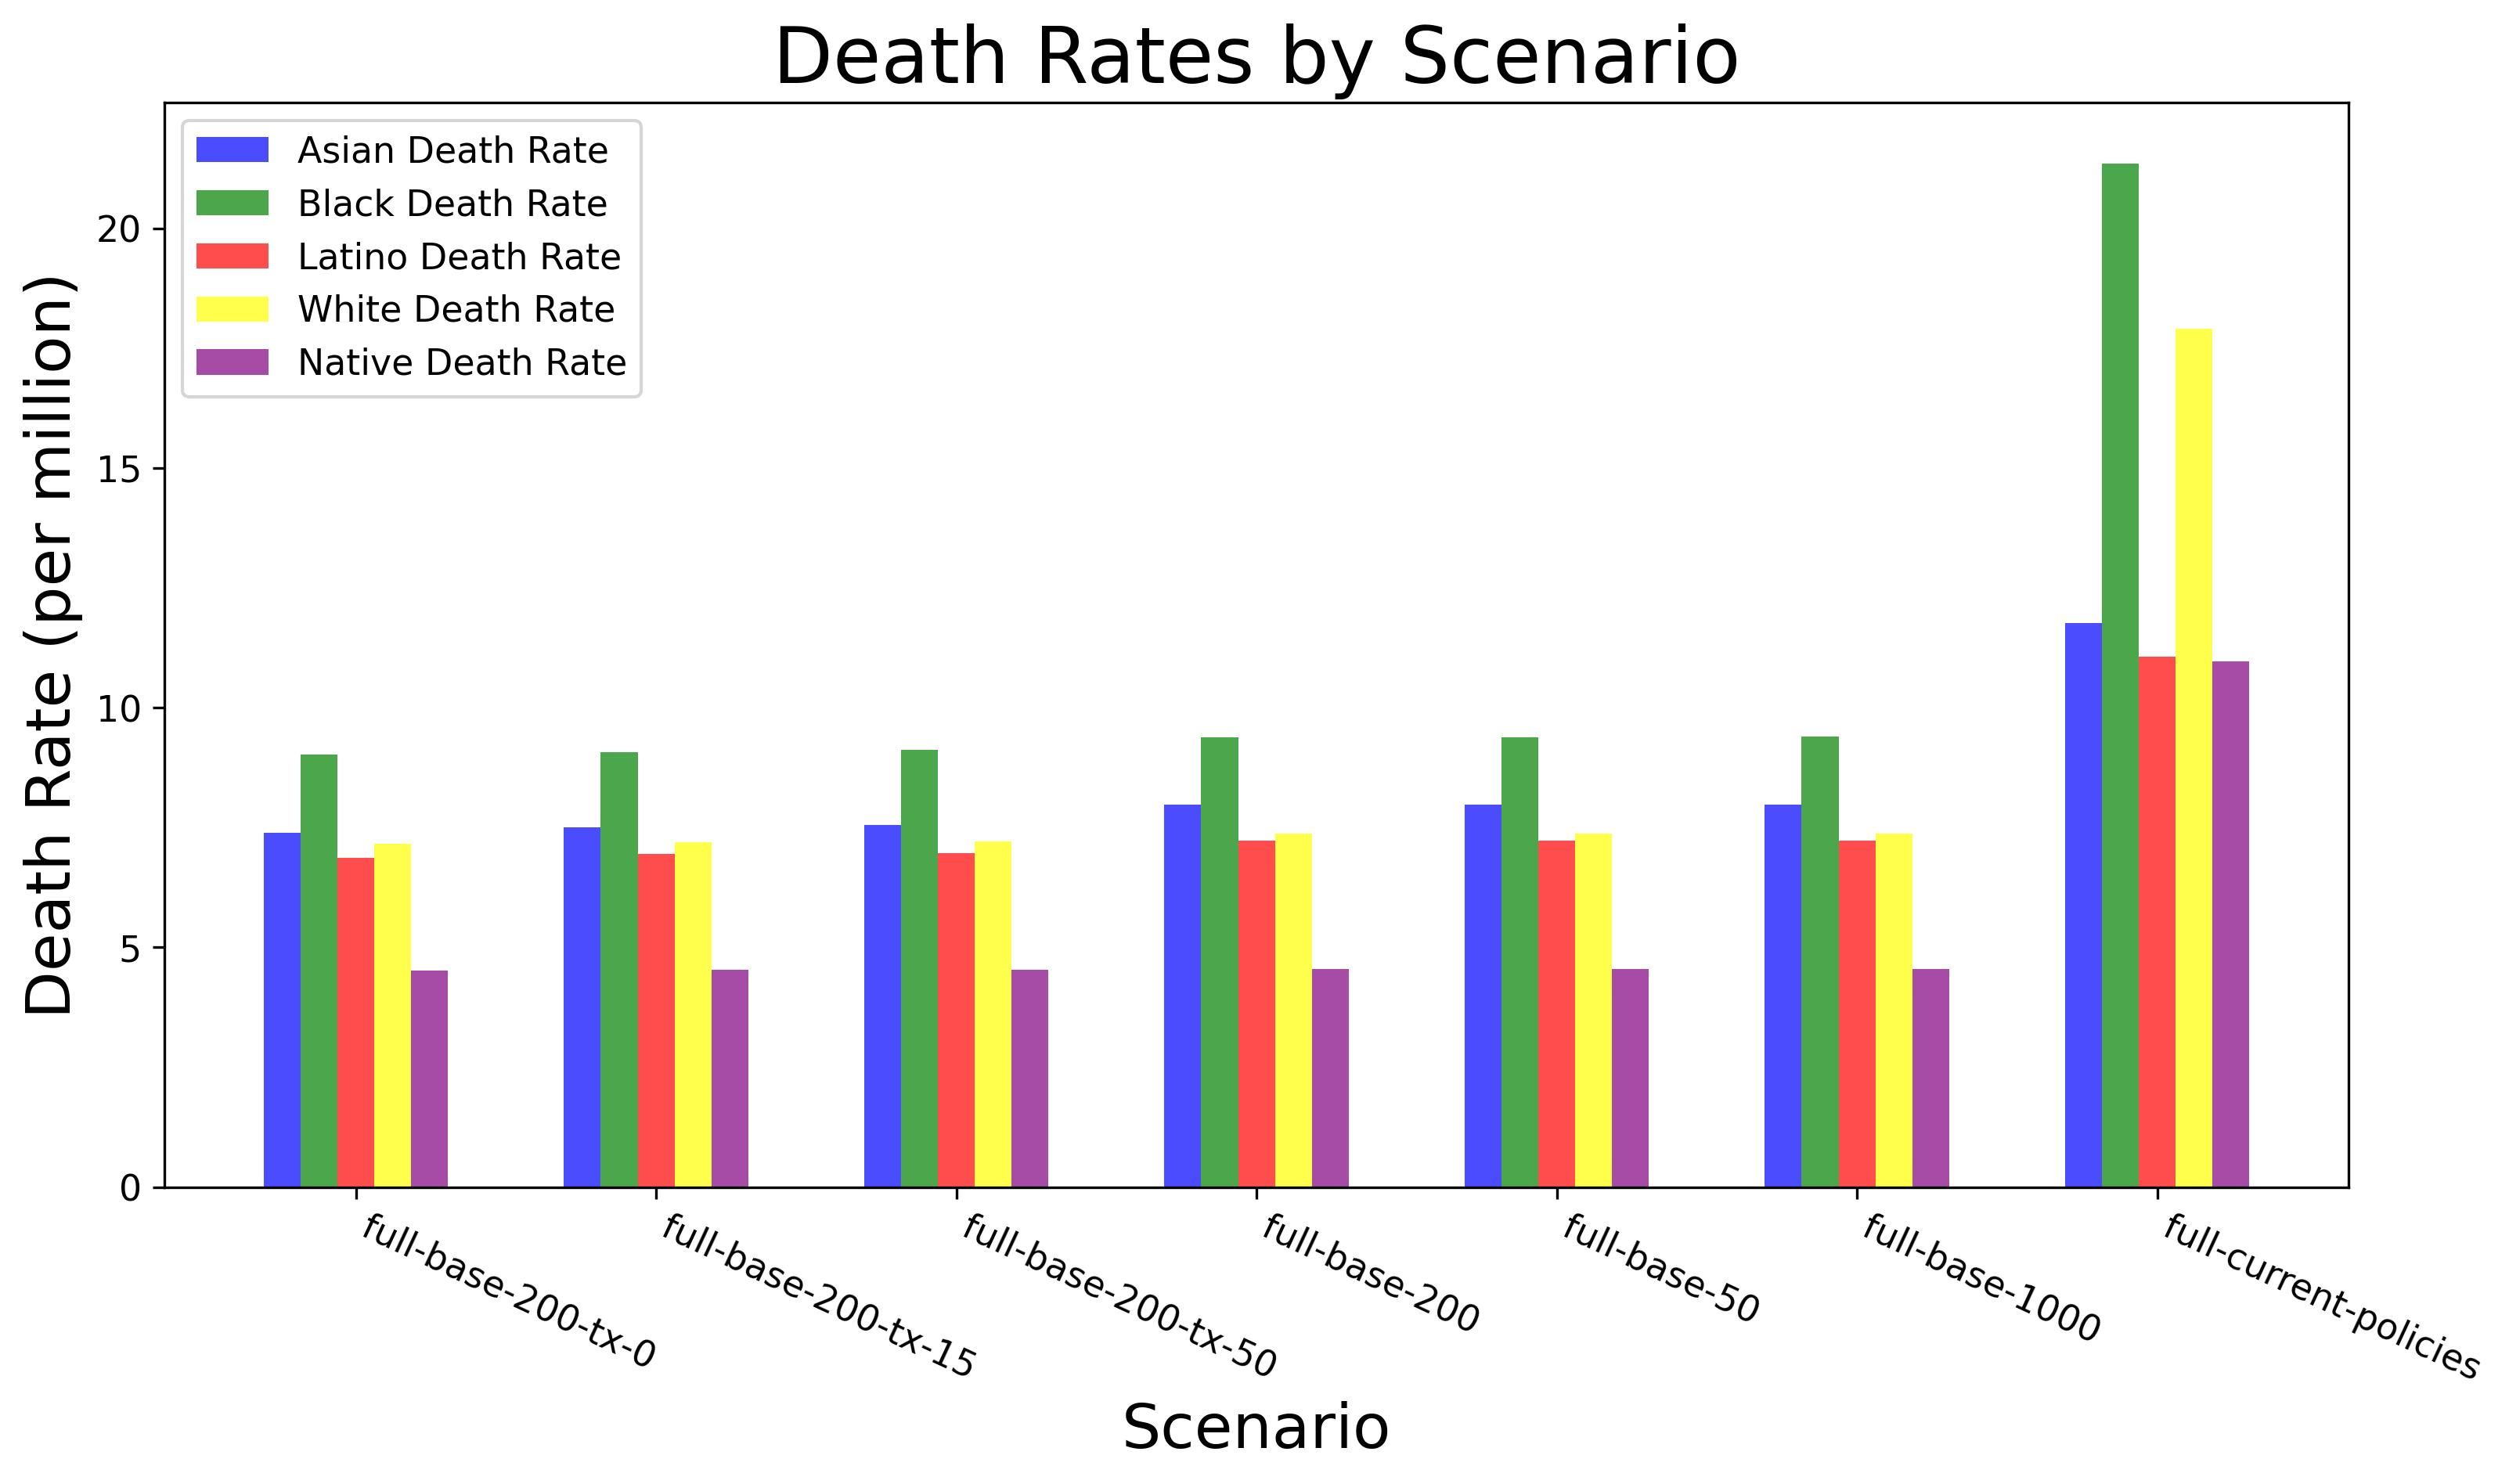
\includegraphics[width=\textwidth]{Figures/Output/Compare_scenarios_all-scenarios_2027_GenX.jpg}
        \caption{2027}
        \label{Subfig1}
    \end{subfigure}
    \hfill
    \begin{subfigure}[b]{0.49\textwidth}
        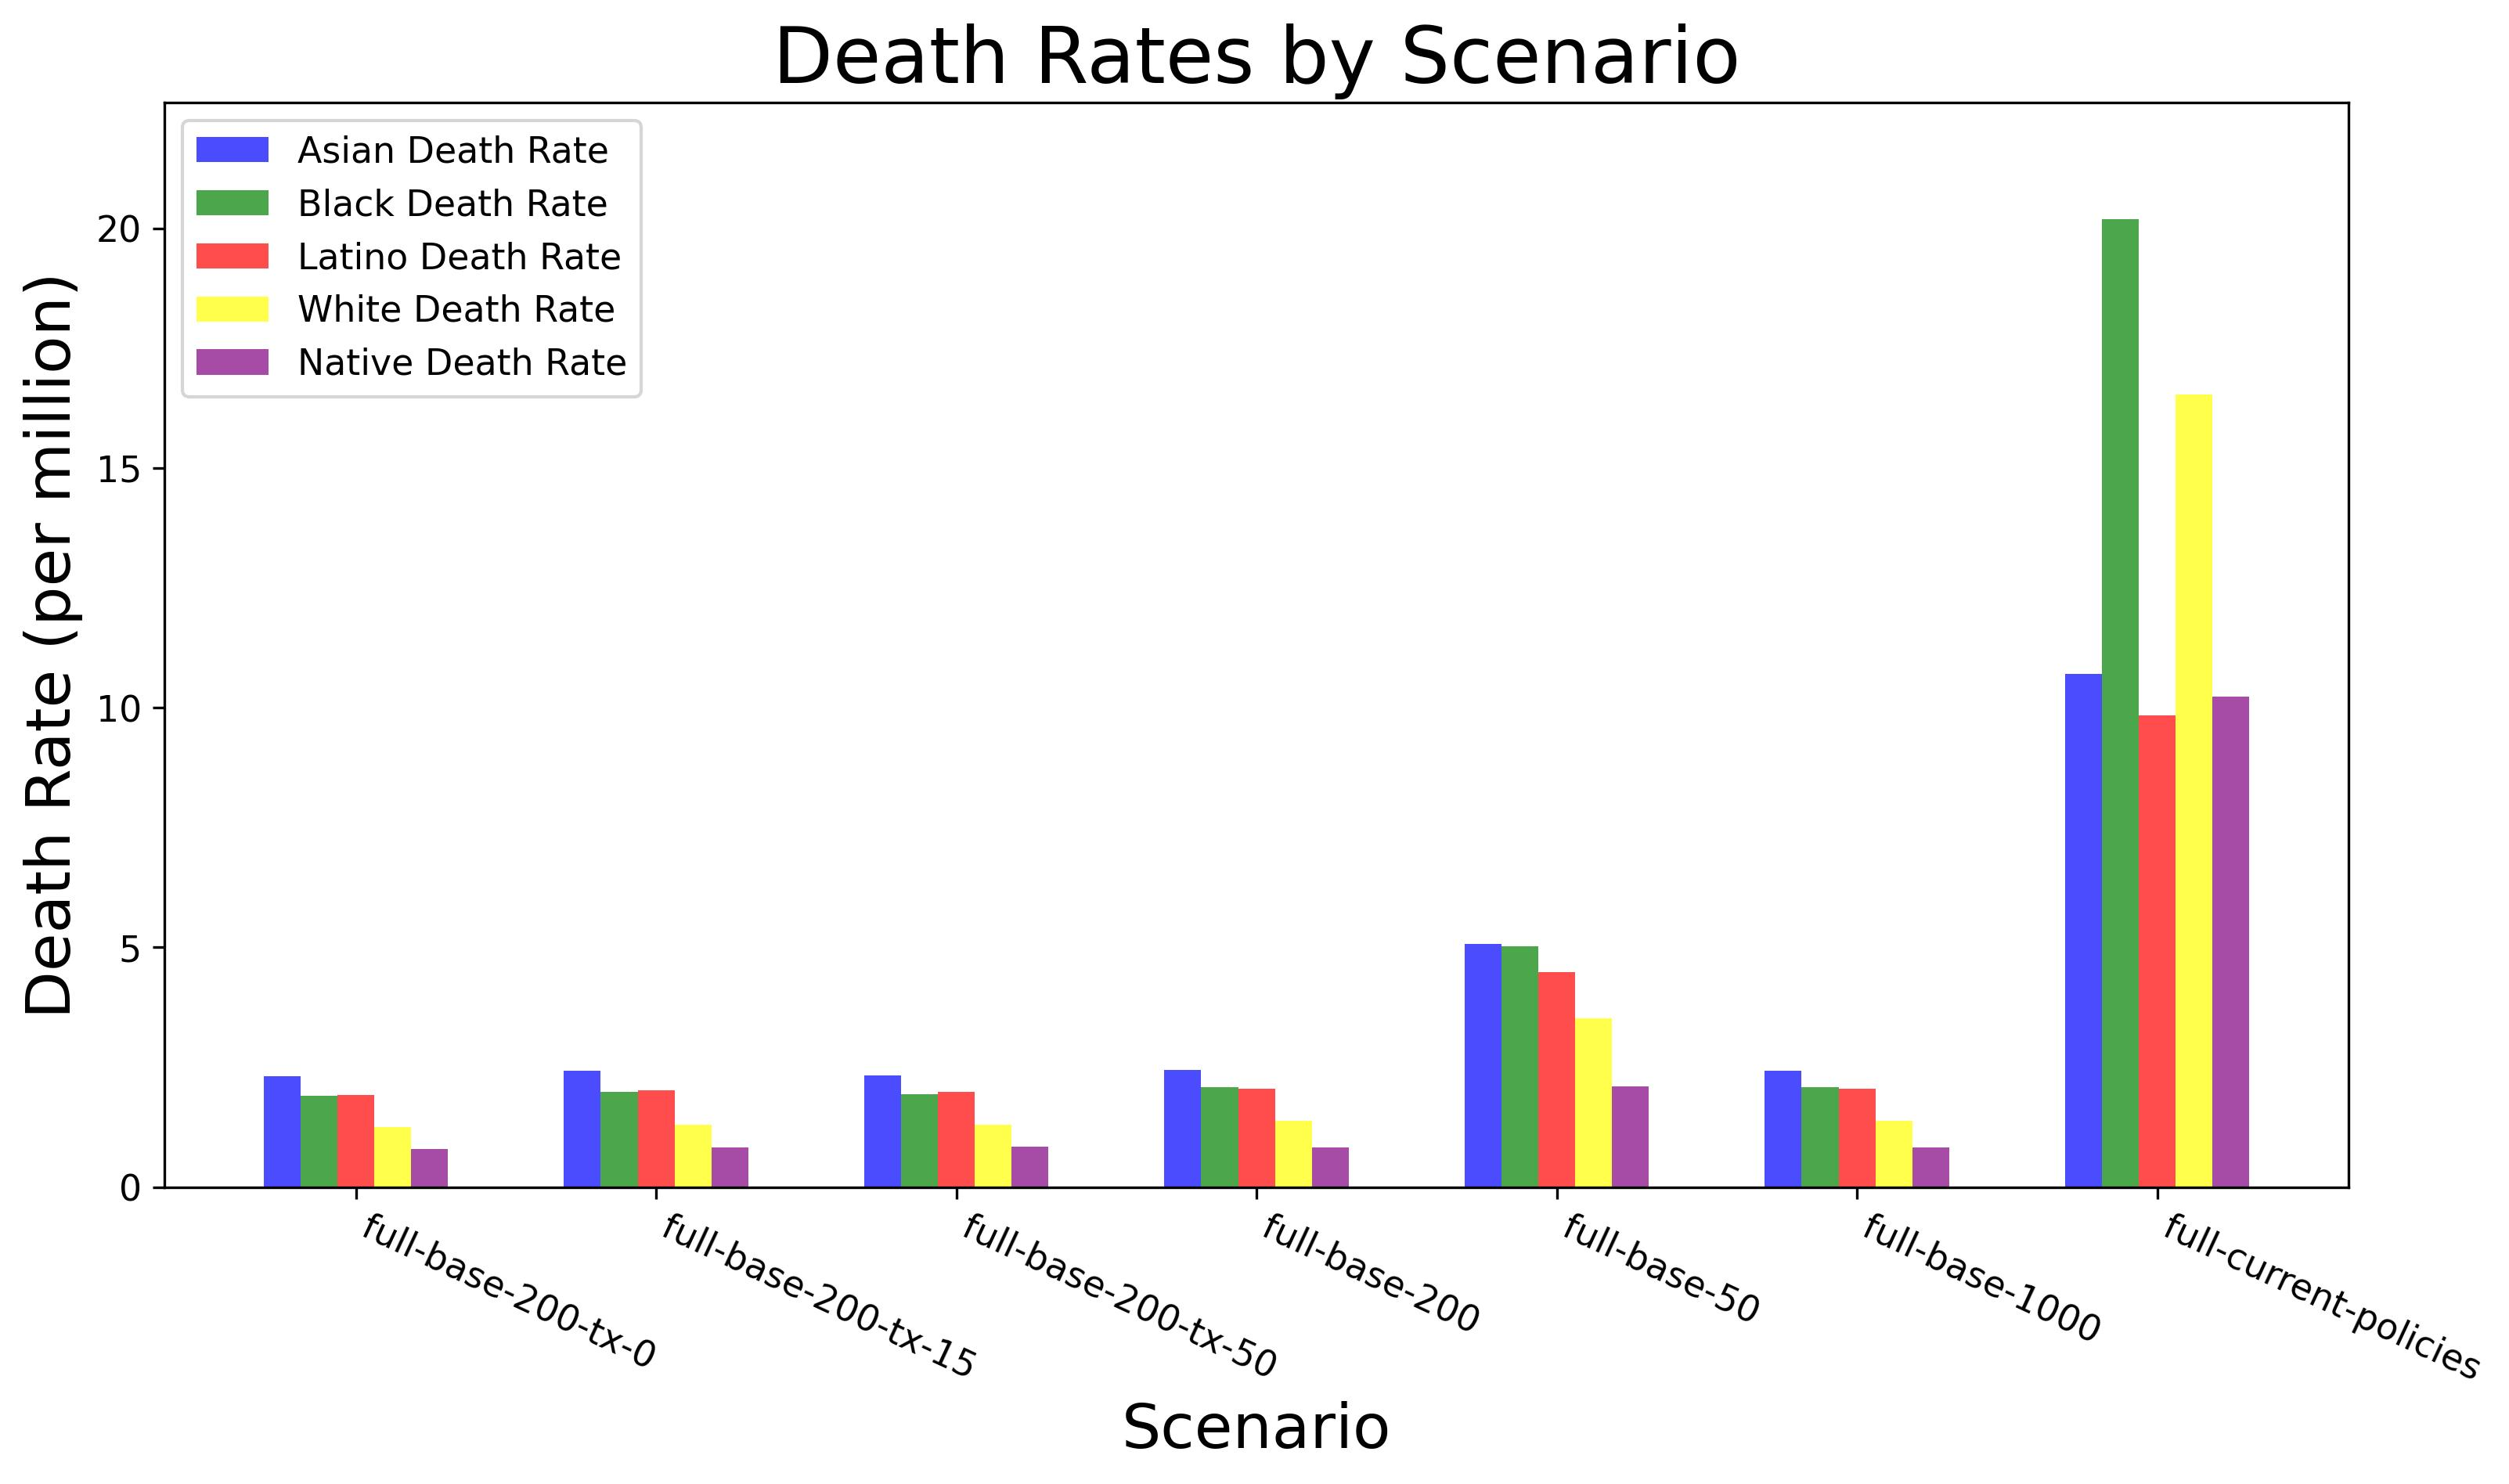
\includegraphics[width=\textwidth]{Figures/Output/Compare_scenarios_all-scenarios_2030_GenX.jpg}
        \caption{2030}
        \label{Subfig2}
    \end{subfigure}\\

        \begin{subfigure}[b]{0.49\textwidth}
        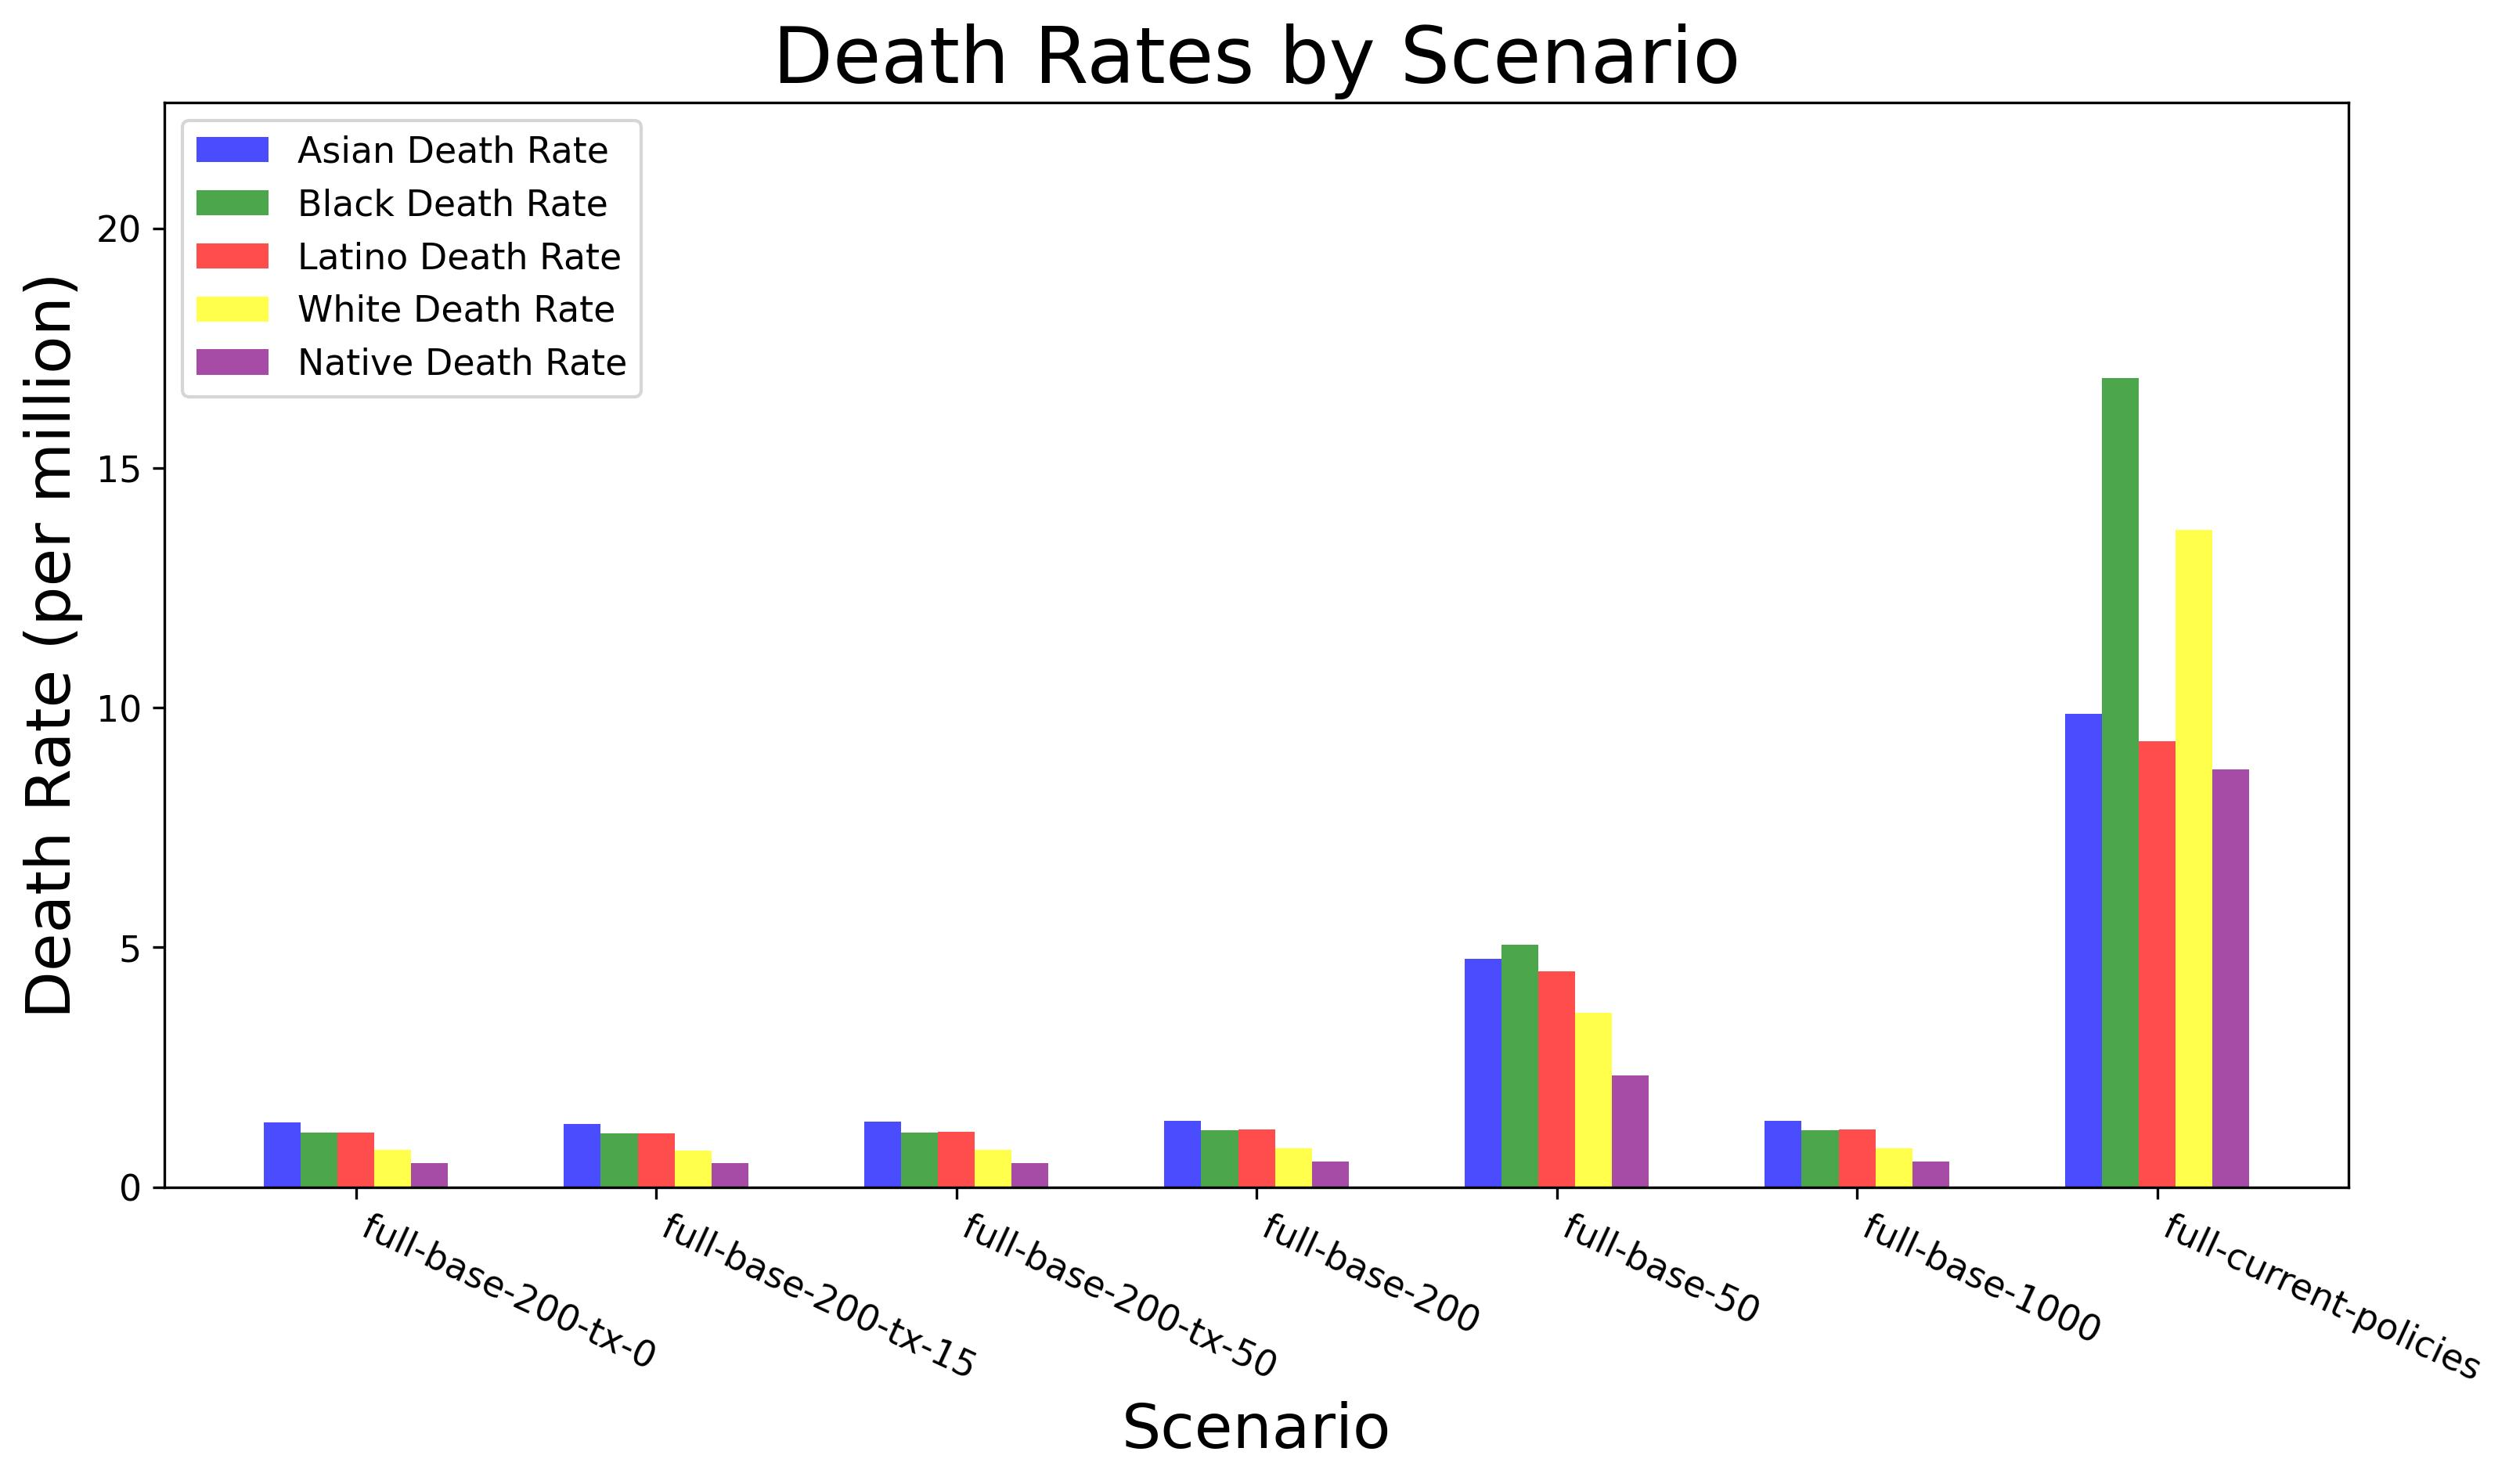
\includegraphics[width=\textwidth]{Figures/Output/Compare_scenarios_all-scenarios_2035_GenX.jpg}
        \caption{2035}
        \label{Subfig2}
    \end{subfigure}
    \hfill
        \begin{subfigure}[b]{0.49\textwidth}
        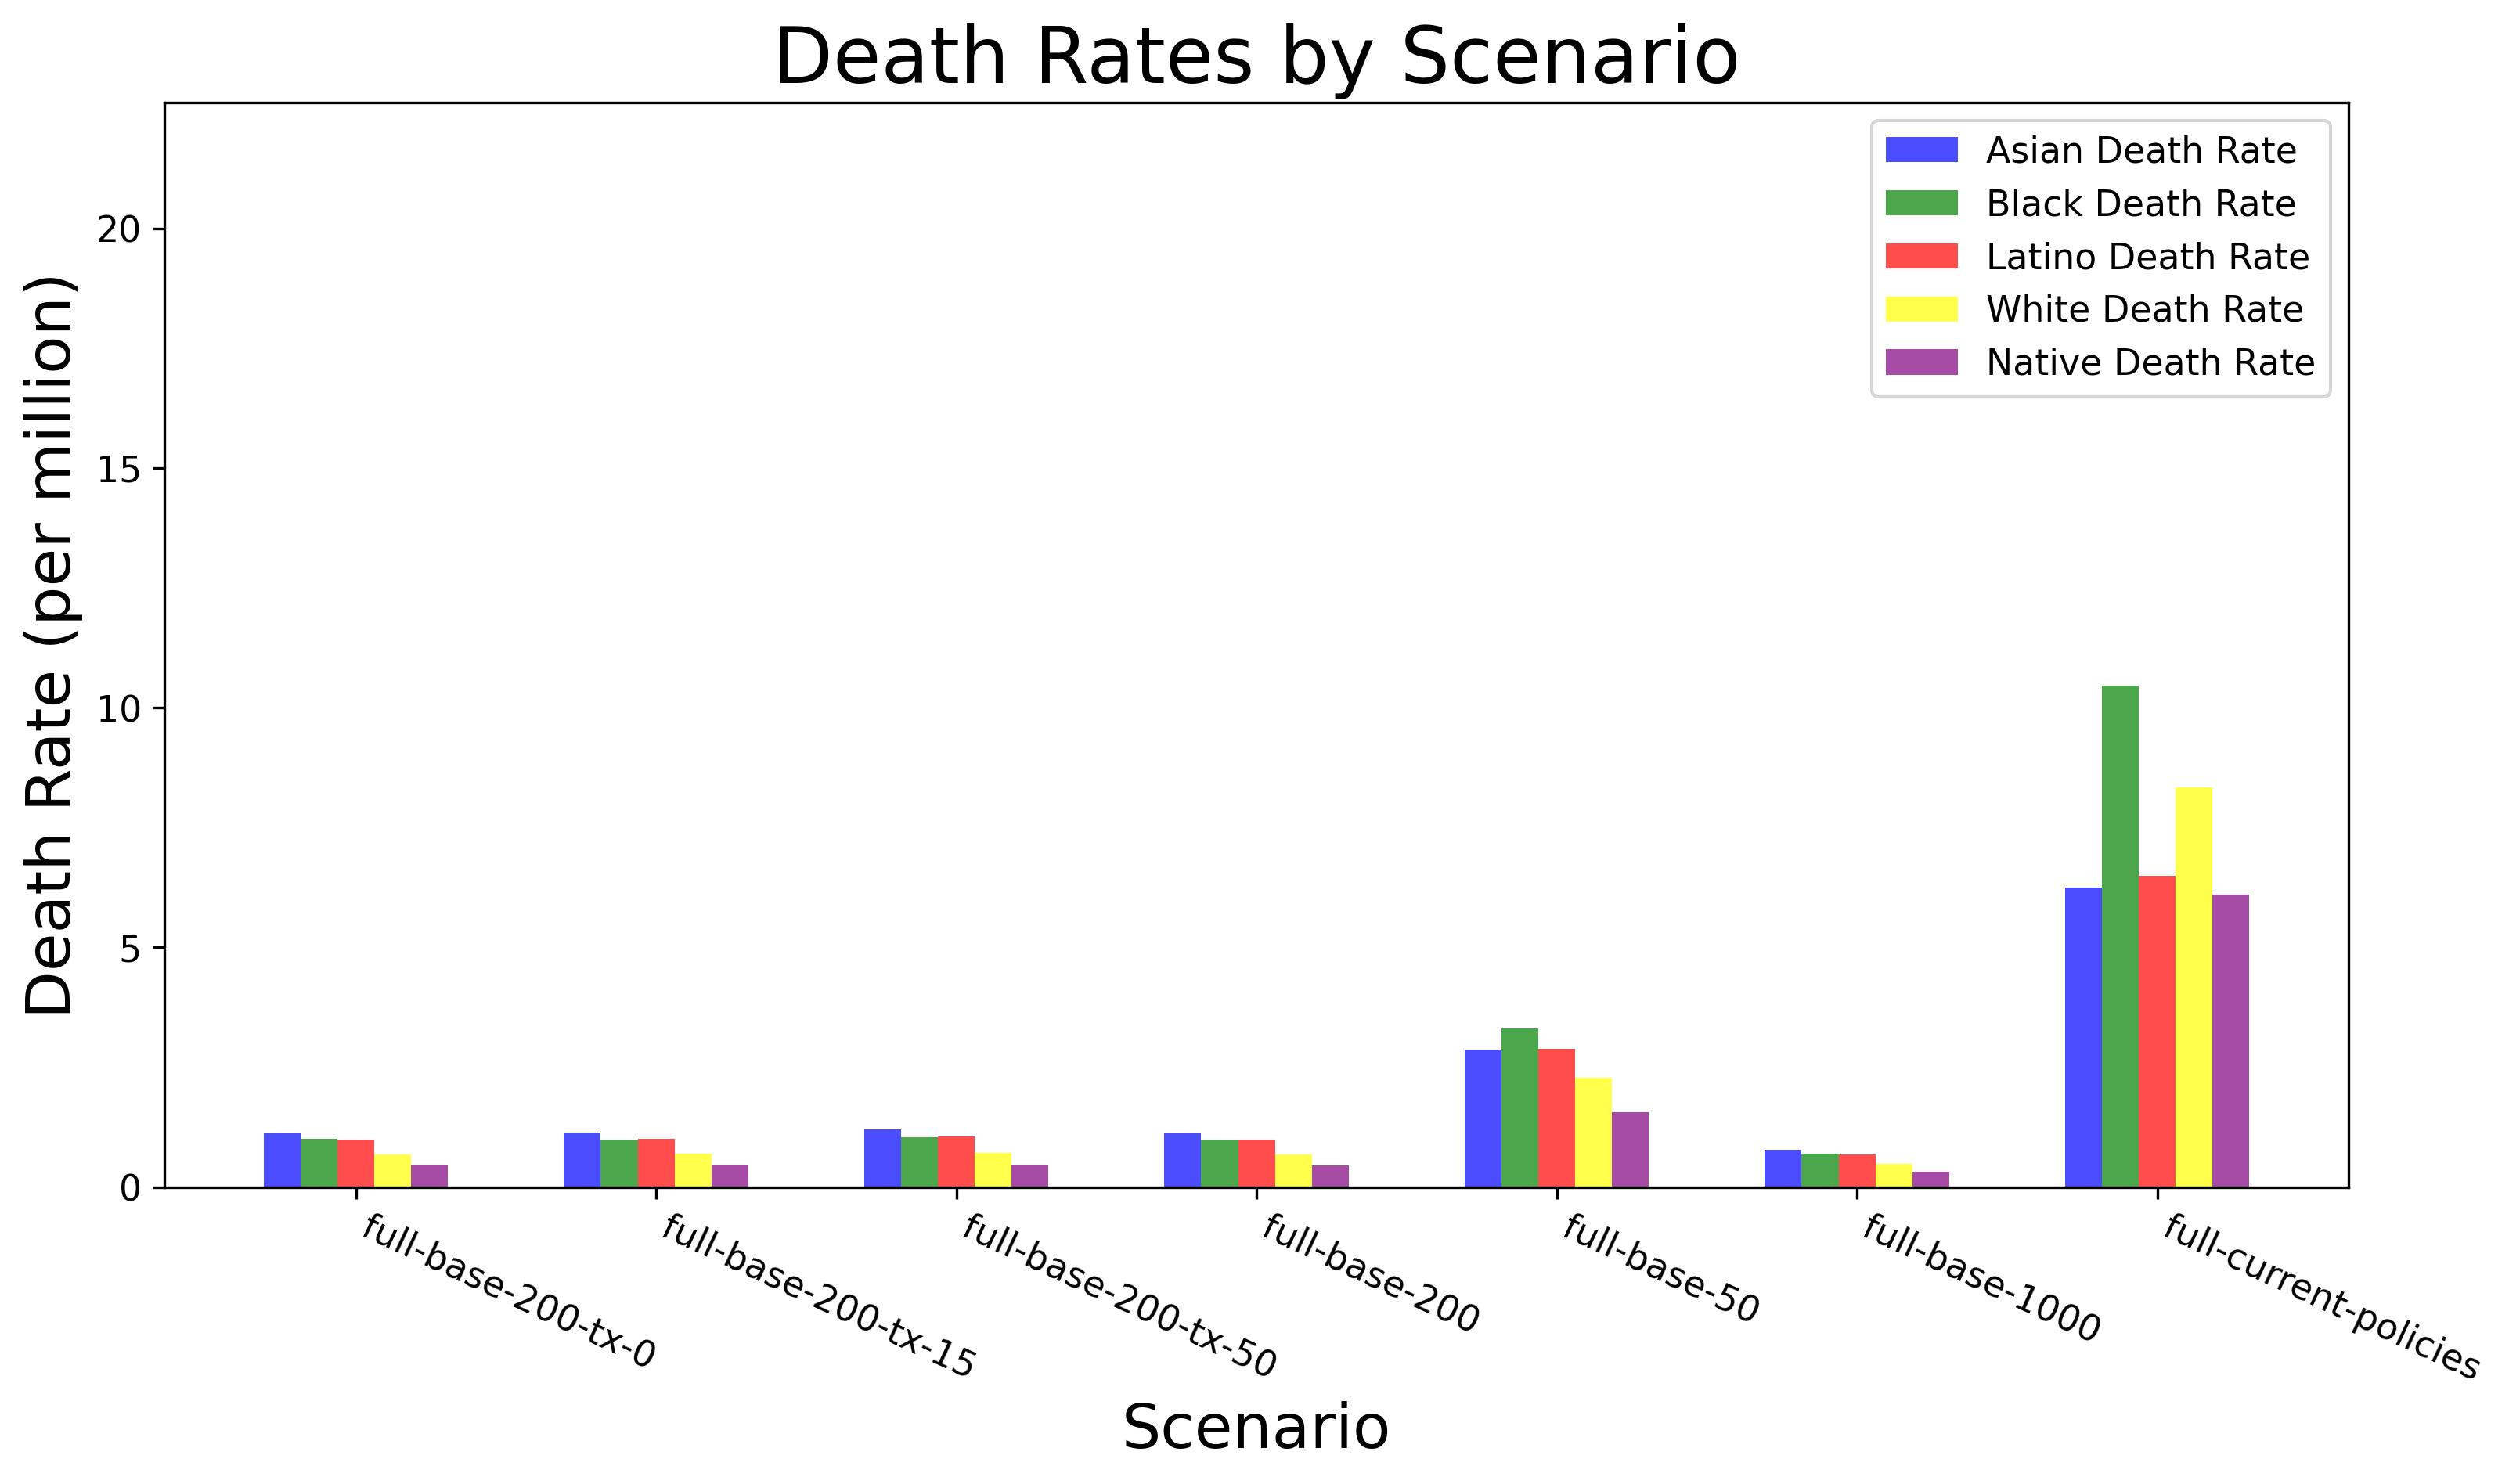
\includegraphics[width=\textwidth]{Figures/Output/Compare_scenarios_all-scenarios_2040_GenX.jpg}
        \caption{2040}
        \label{Subfig2}
    \end{subfigure}\\

    \begin{subfigure}[b]{0.49\textwidth}
        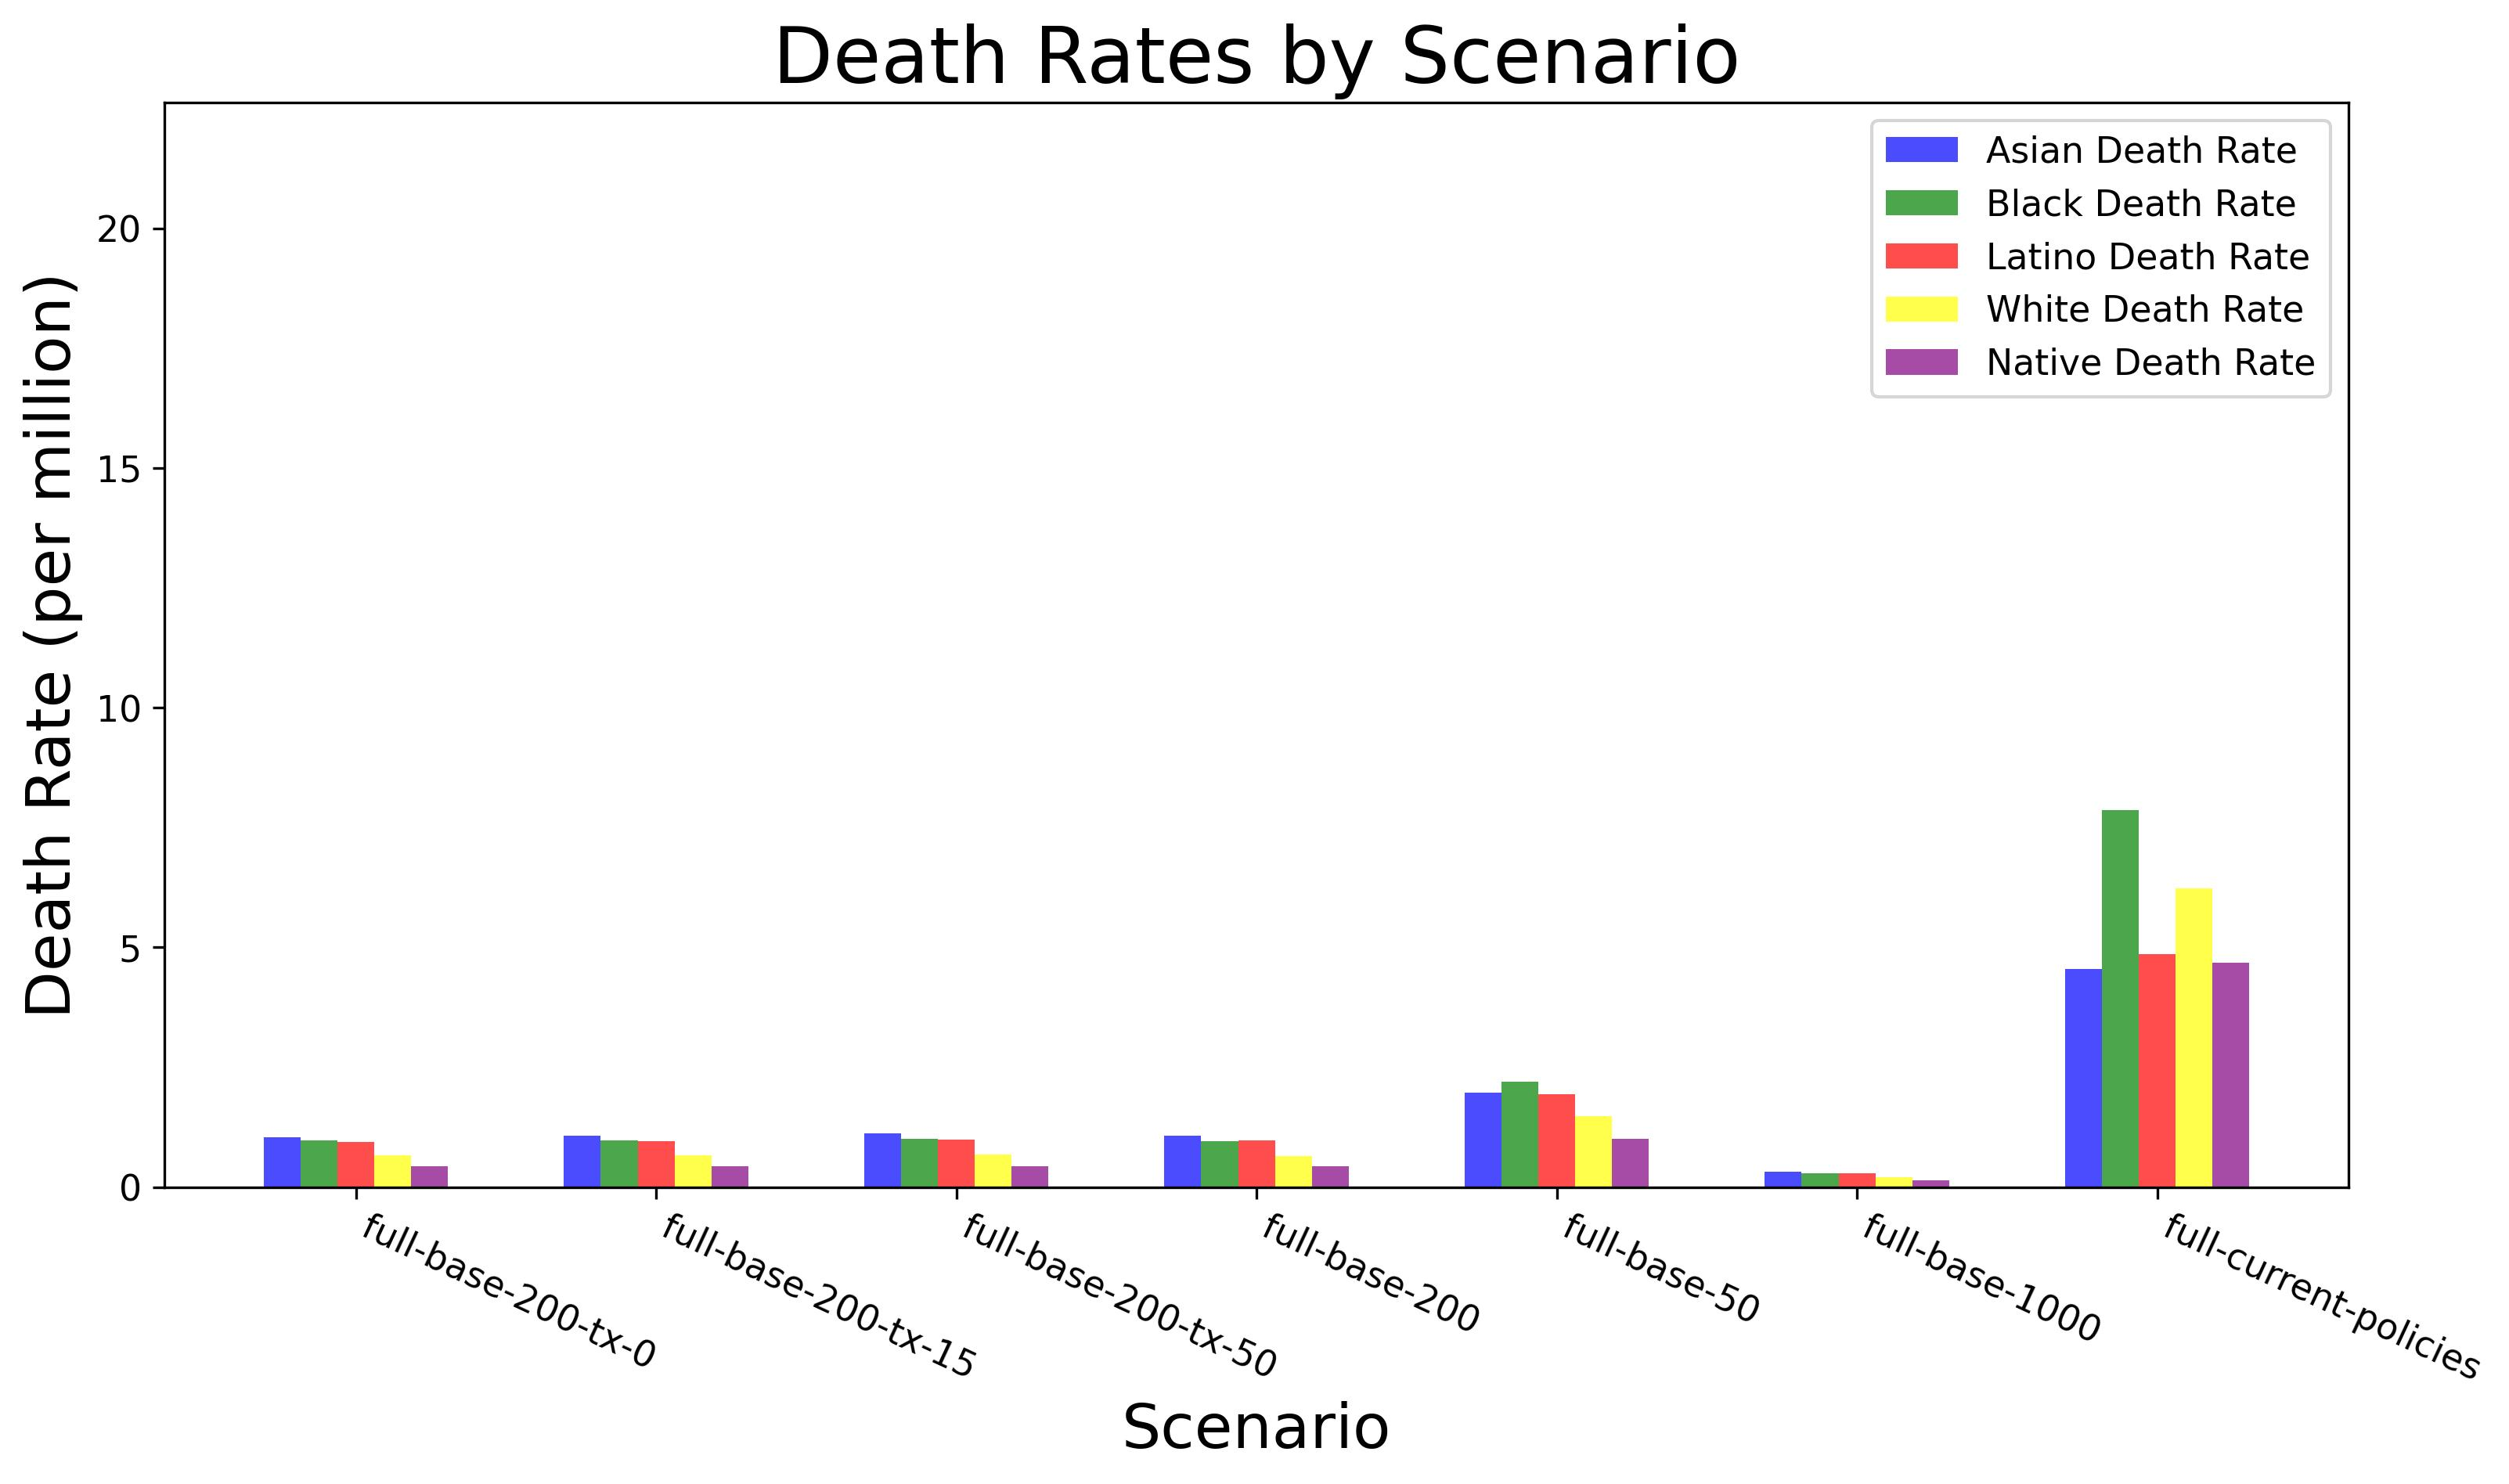
\includegraphics[width=\textwidth]{Figures/Output/Compare_scenarios_all-scenarios_2045_GenX.jpg}
        \caption{2045}
        \label{Subfig2}
    \end{subfigure}
    \hfill
    \begin{subfigure}[b]{0.49\textwidth}
        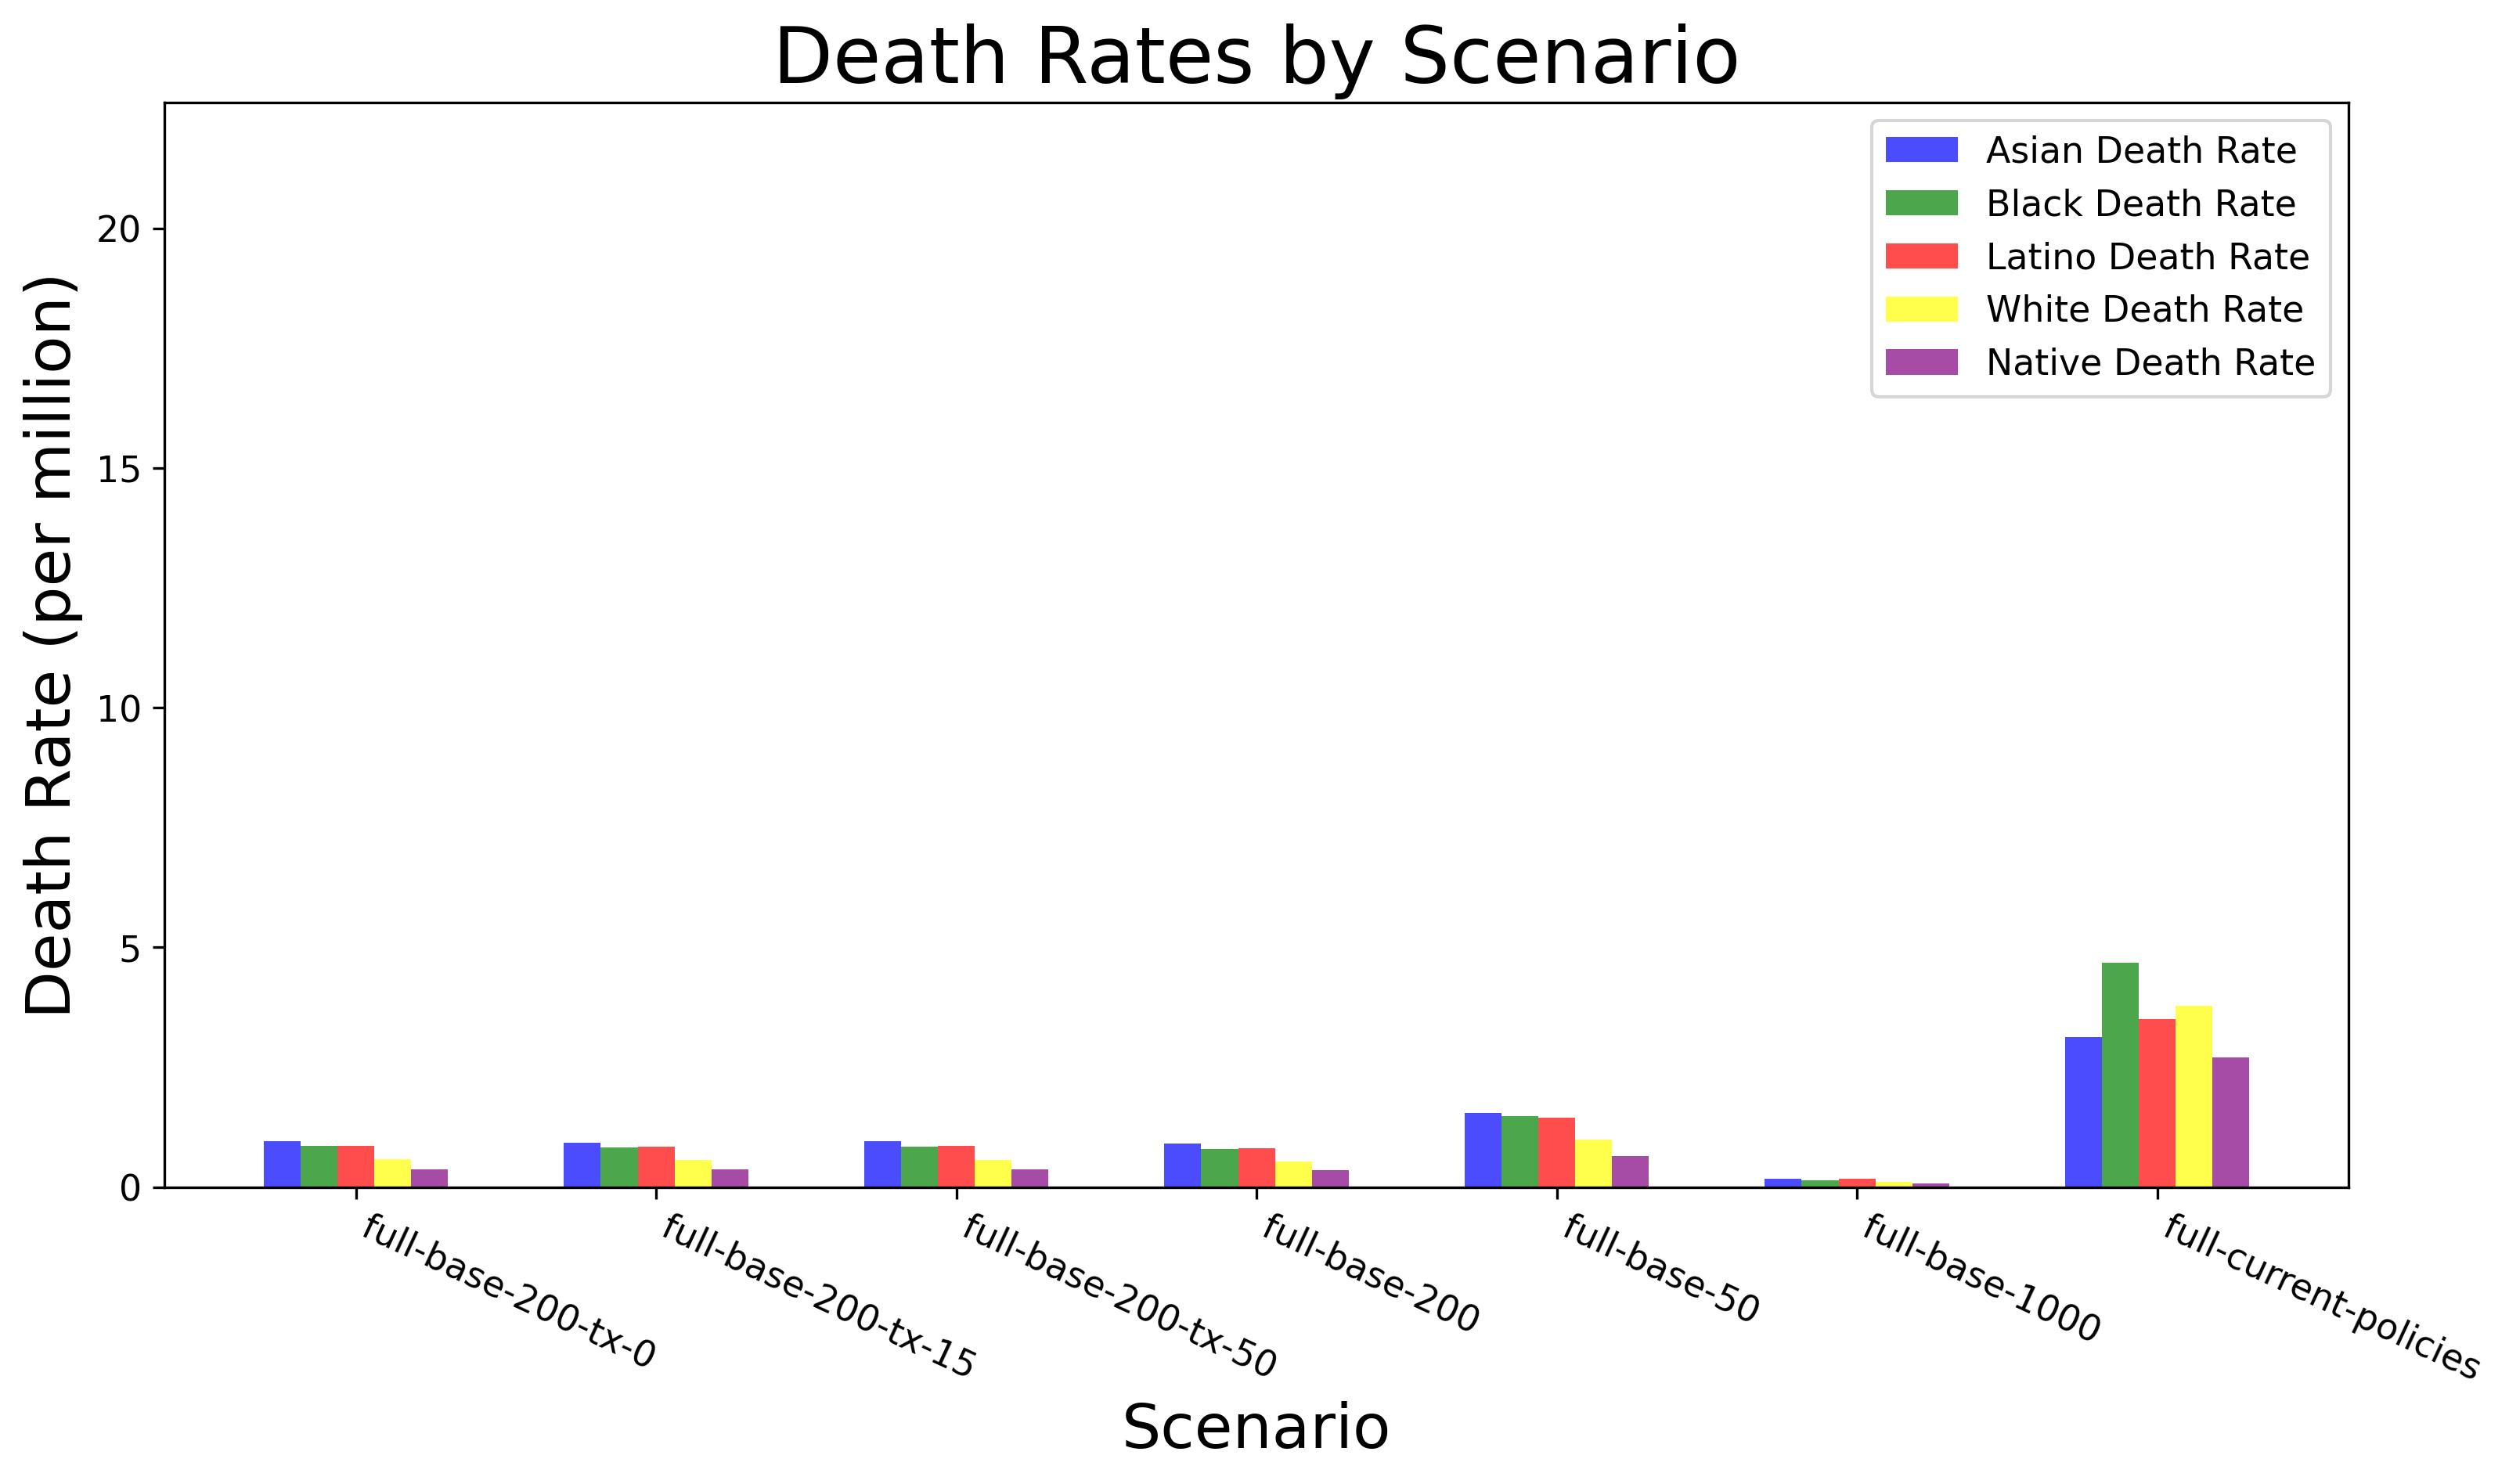
\includegraphics[width=\textwidth]{Figures/Output/Compare_scenarios_all-scenarios_2050_GenX.jpg}
        \caption{2050}
        \label{Subfig2}
    \end{subfigure}
    \caption{Comparison results by scenario over time}
    \label{Compare Scenarios}
\end{figure}

In figure \ref{DeathsCosts} we plot deaths against total system costs.  The policies that seemingly do the best in terms of cost-effectiveness are the full-base-200 scenarios.  NOTE FOR DISCUSSION -- THIS IS ALMOST BY CONSTRUCTION SINCE CO2 COSTS ARE INCLUDED IN TOTAL COSTS
\begin{figure}
    \centering
    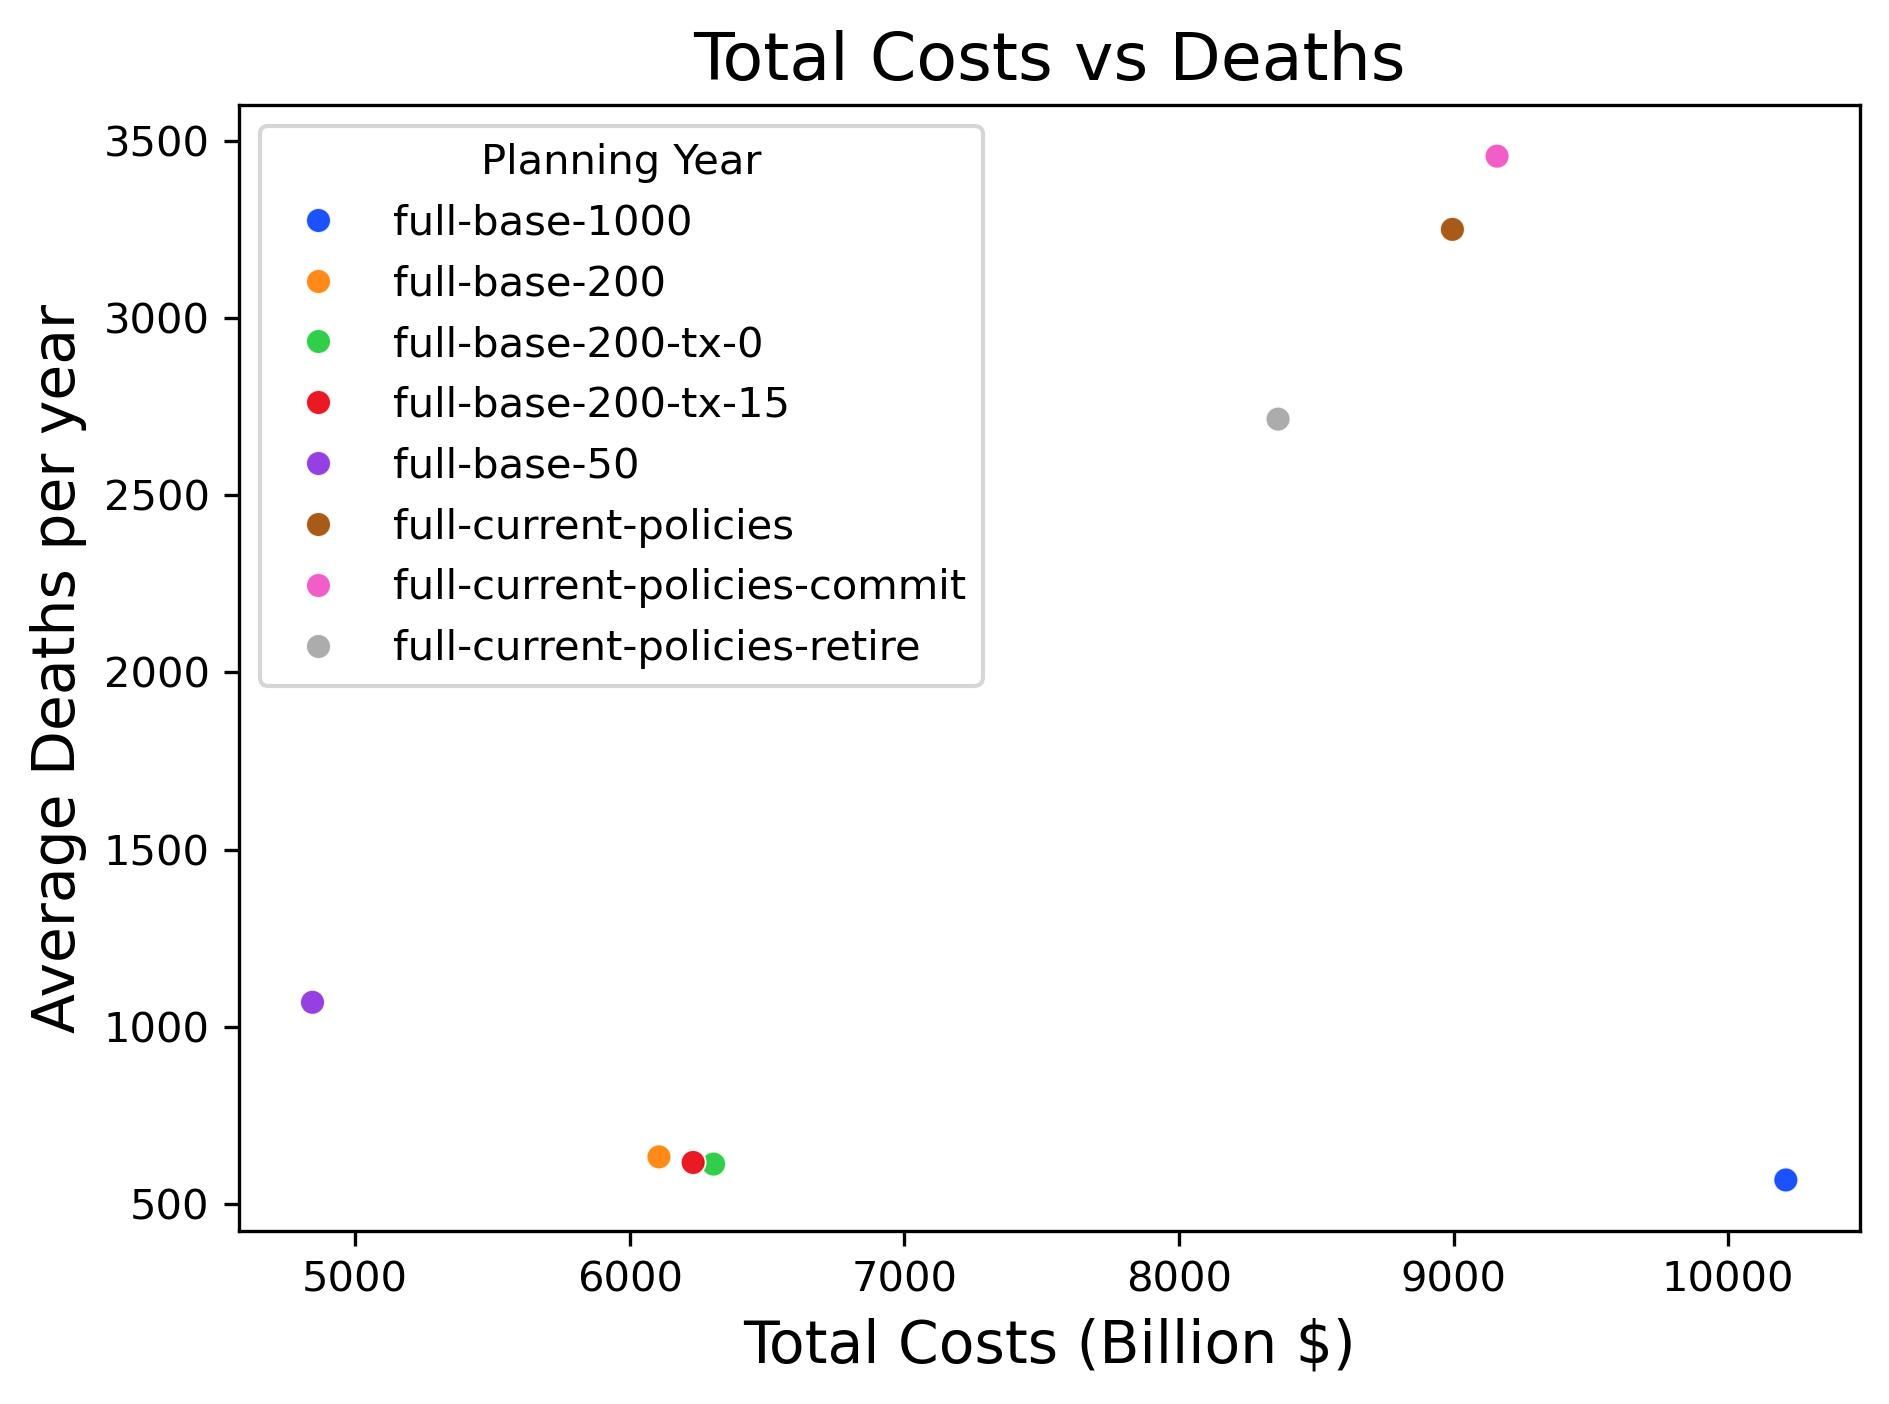
\includegraphics[width=0.8\linewidth]{Figures/Output/Deaths_vs_Costs_GenX.png}
    \caption{Plot of total system costs versus average deaths per year.  Results are from GenX output.}
    \label{DeathsCosts}
\end{figure}

Unsurprisingly, deaths are highly correlated with CO$_2$ emissions, since both are driven by fossil-fuel combustion.  Policies that most dramatically reduce CO$_2$ emissions, also do the most to reduce aggregate deaths.
\begin{figure}
    \centering
    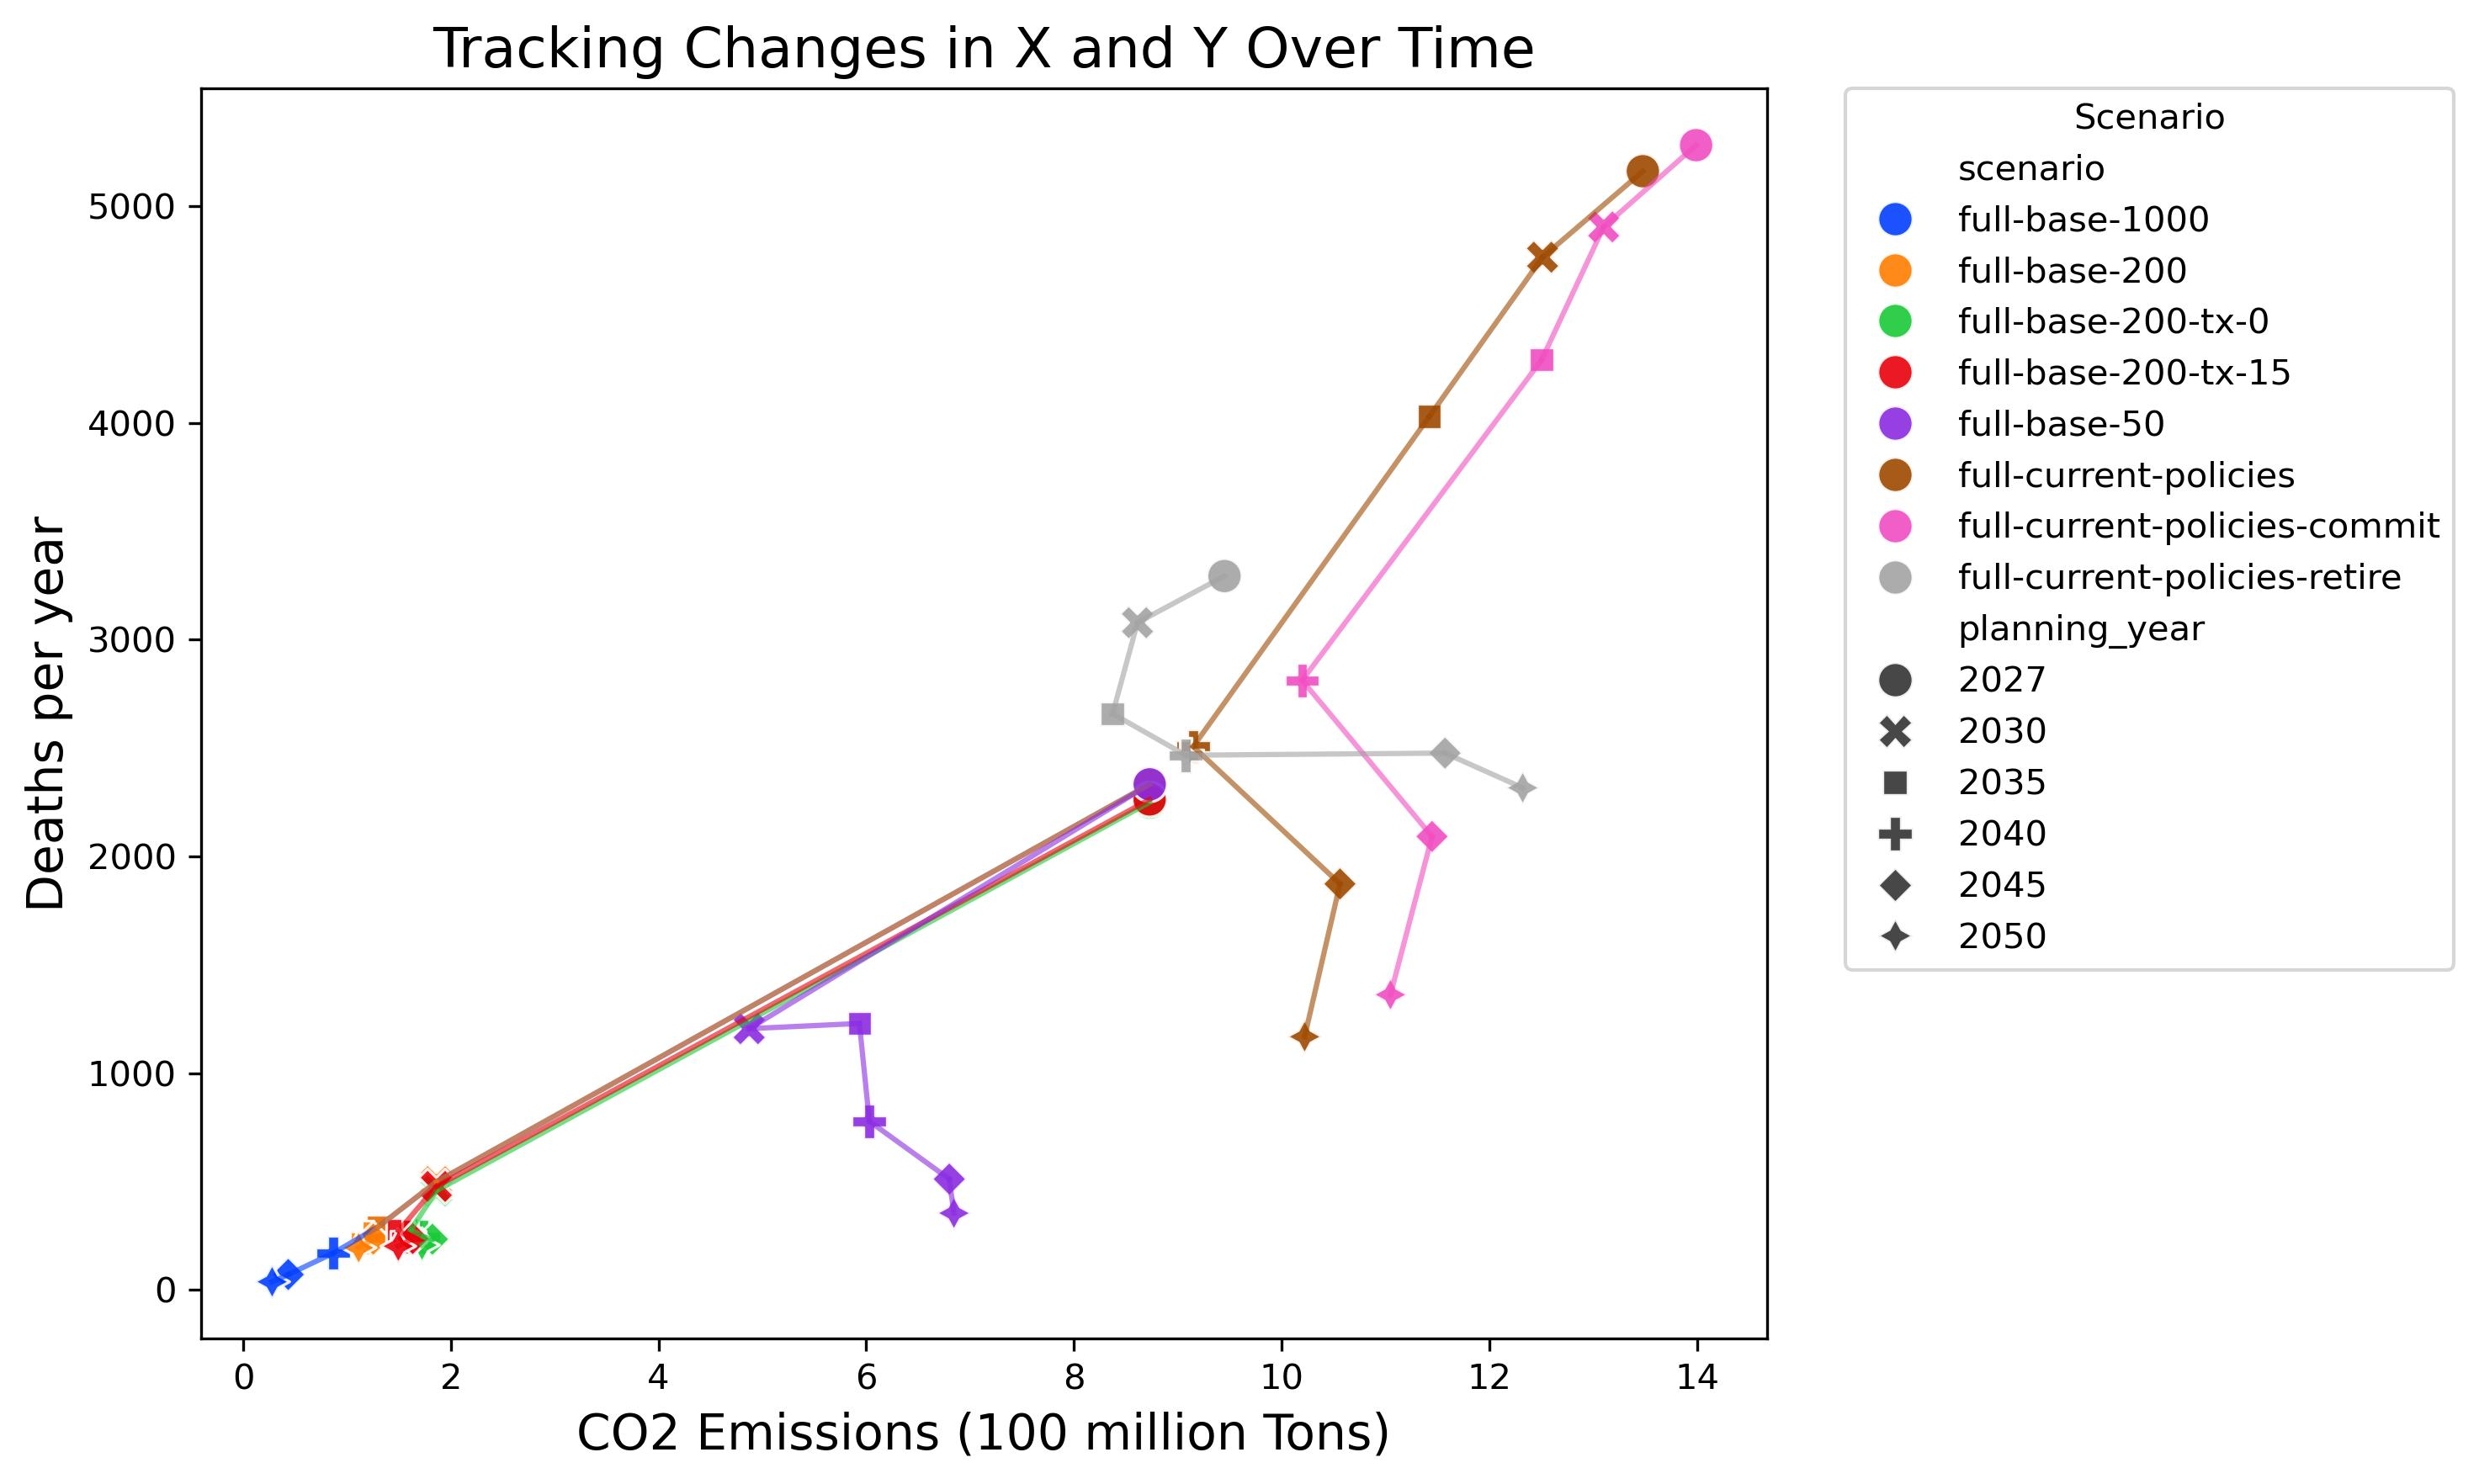
\includegraphics[width=1\linewidth]{Figures/Output/Deaths_vs_Emissions_withlines_GenX.png}
    \caption{Deaths are highly correlated with CO$_2$ emissions.  In this plot, points are colored by scenarios and shaped by model year.  We also draw lines to show the trajectory over time for each model.}
    \label{DeathsEmissions}
\end{figure}

These results mirror previous related work.  \citet{Shawhan2024PoliciesAmericans} found that a carbon tax would decrease deaths by X$\%$.  \citet{Goforth2022AirStrategies} find that THINGS.

\subsection{Varying the Escape Price}
In figure \ref{EscapePrice} we plot death rates over time across different escape-price scenarios.  The difference between a $\$50$ escape price and a $\$200$ escape price is quite striking.  However, the change from $\$200$ to $\$1,000$ is far more subtle, and mostly shows up in 2040 and beyond.

\begin{figure}
    \centering
    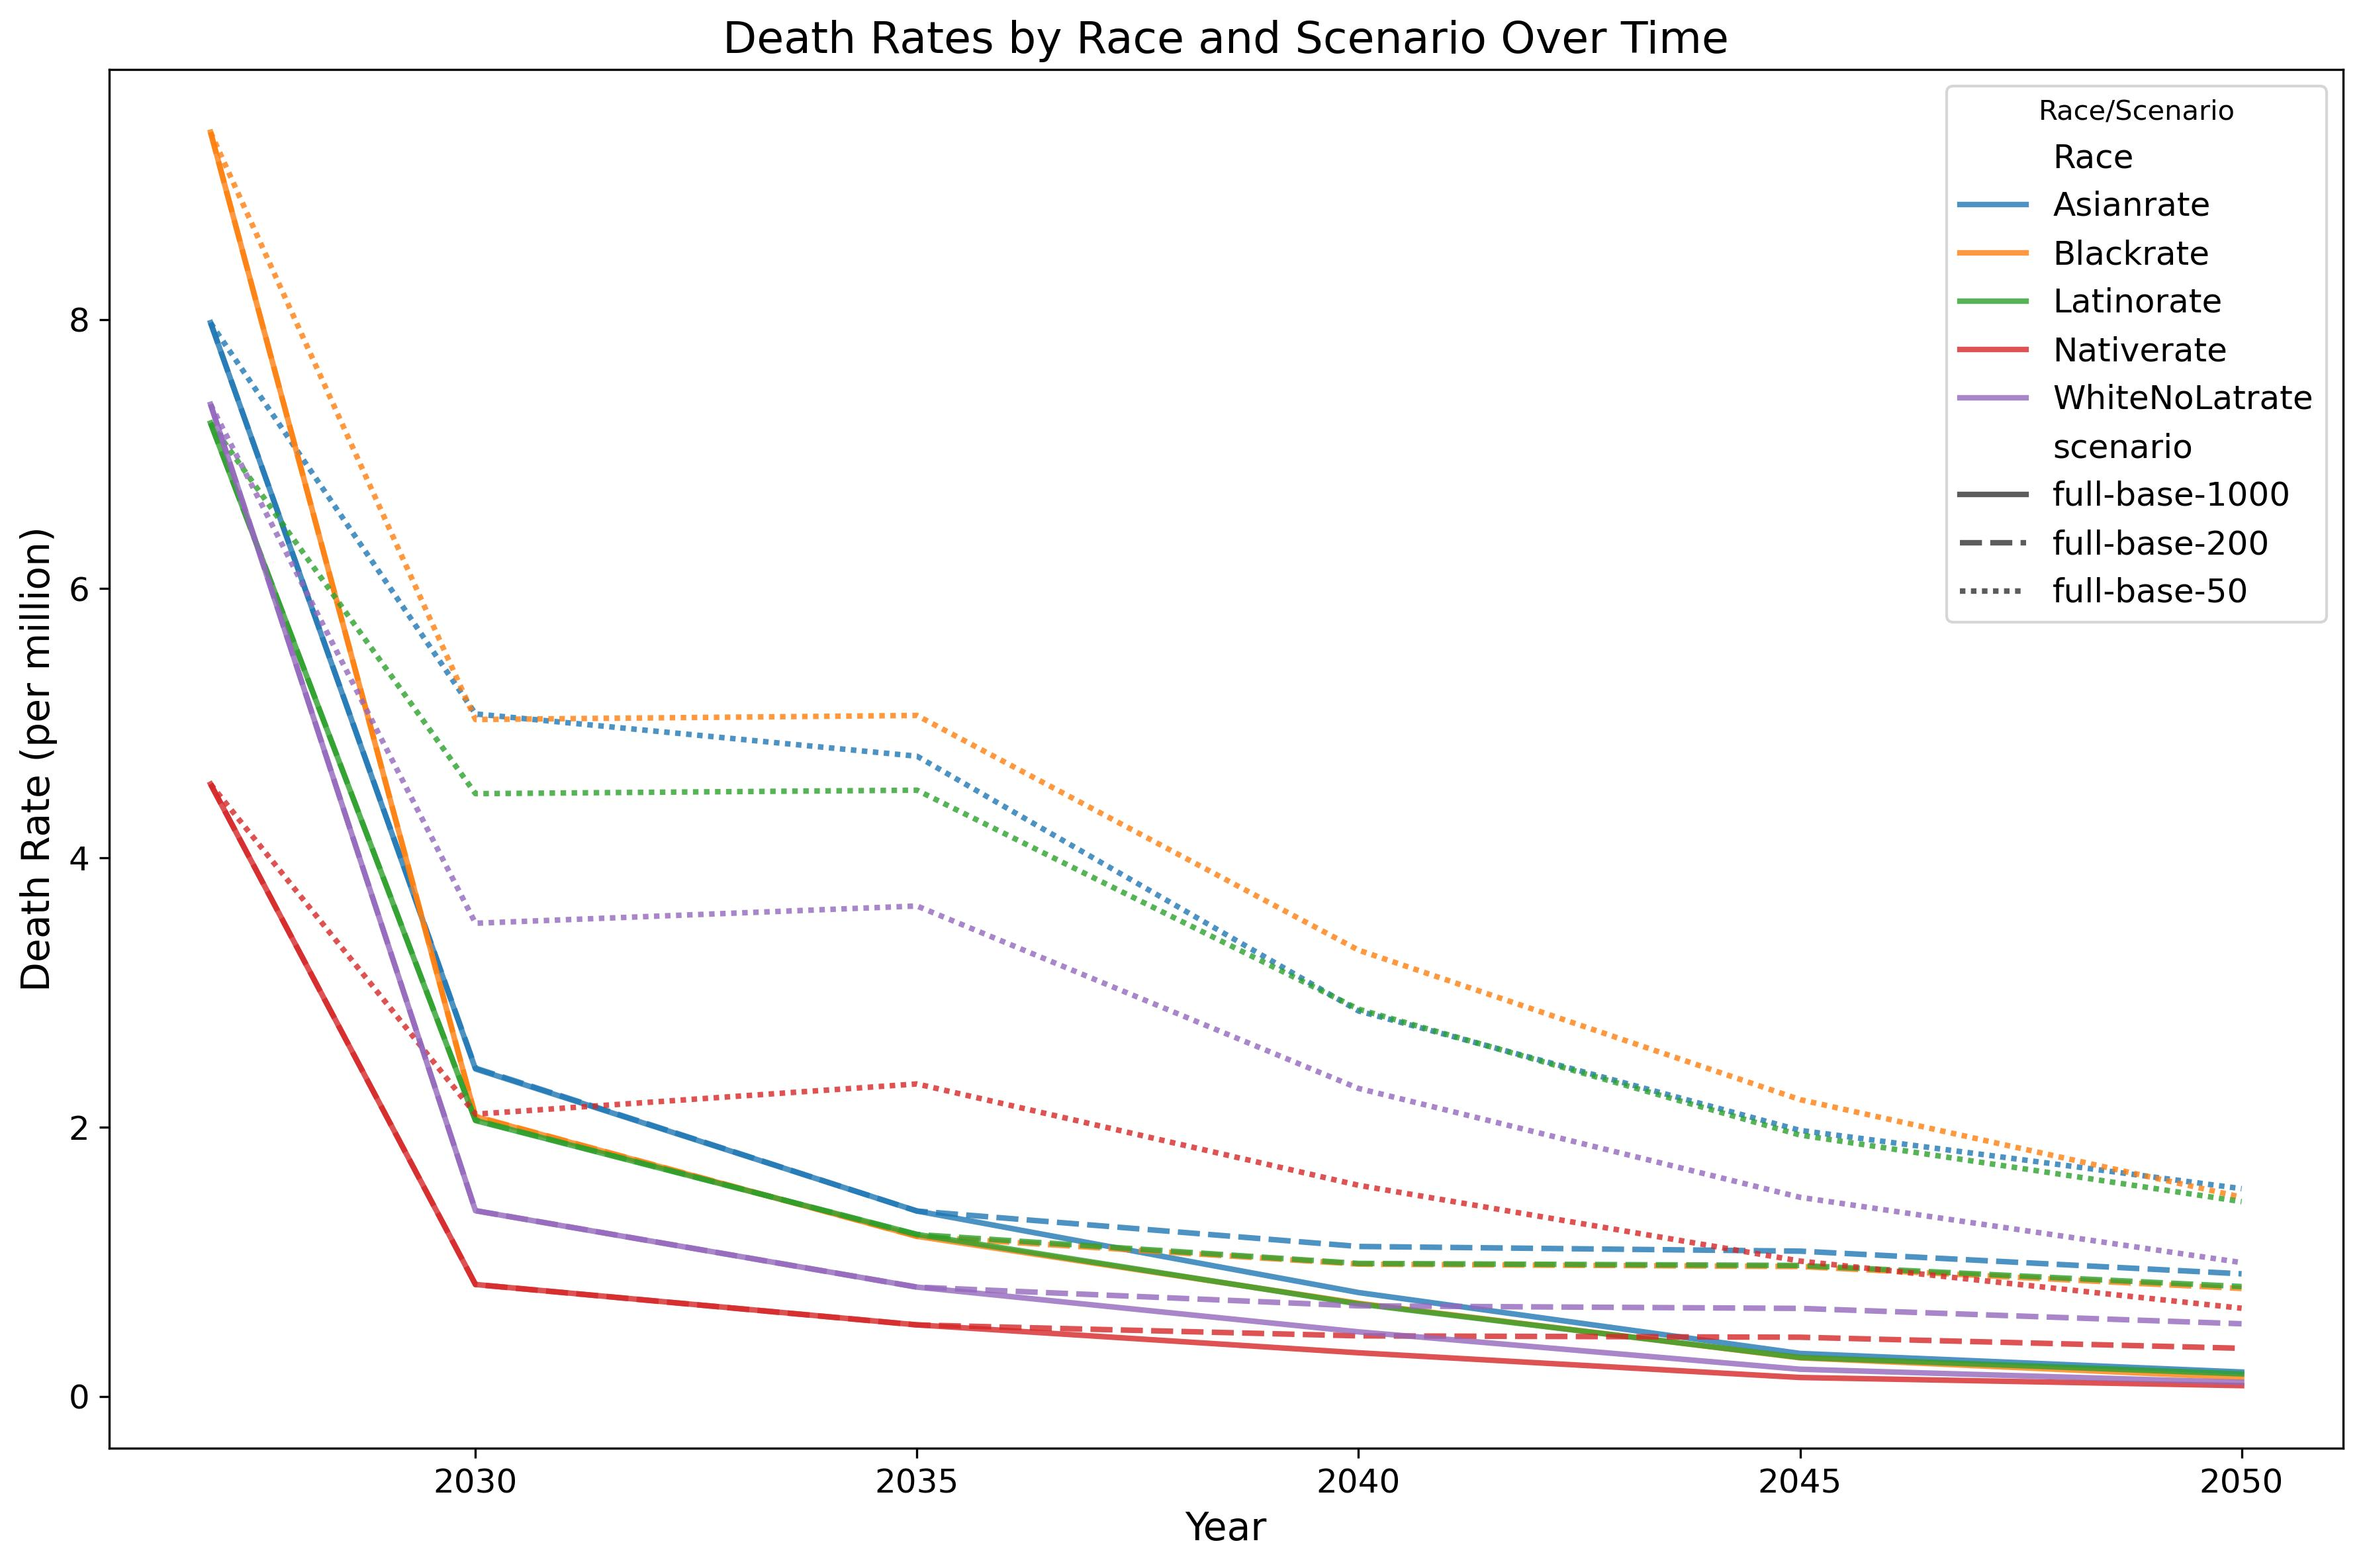
\includegraphics[width=1\linewidth]{Figures/Output/Compare_scenarios_compare-escape-price_GenX.jpg}
    \caption{Death rates over time across escape-price scenarios}
    \label{EscapePrice}
\end{figure}

\subsection{Constraining Transmission Expansion}
In figure \ref{TransmissionConstraint} we plot death rates over time across the transmission constraint scenarios. Transmission constraints appear to have almost no effect on deaths.  As explored in MIP PAPER, the effects of transmission constraints are mostly localized.  MIP PAPER found that while the transmission constraint did not have a major effect on system costs, it did increase aggregate emissions by $X\%$.  The effects on aggregate deaths are far more muted.  The most severe transmission constraint (zero new inter-regional transmission) only has X more deaths per year than the completely unconstrained scenario.
\begin{figure}
    \centering
    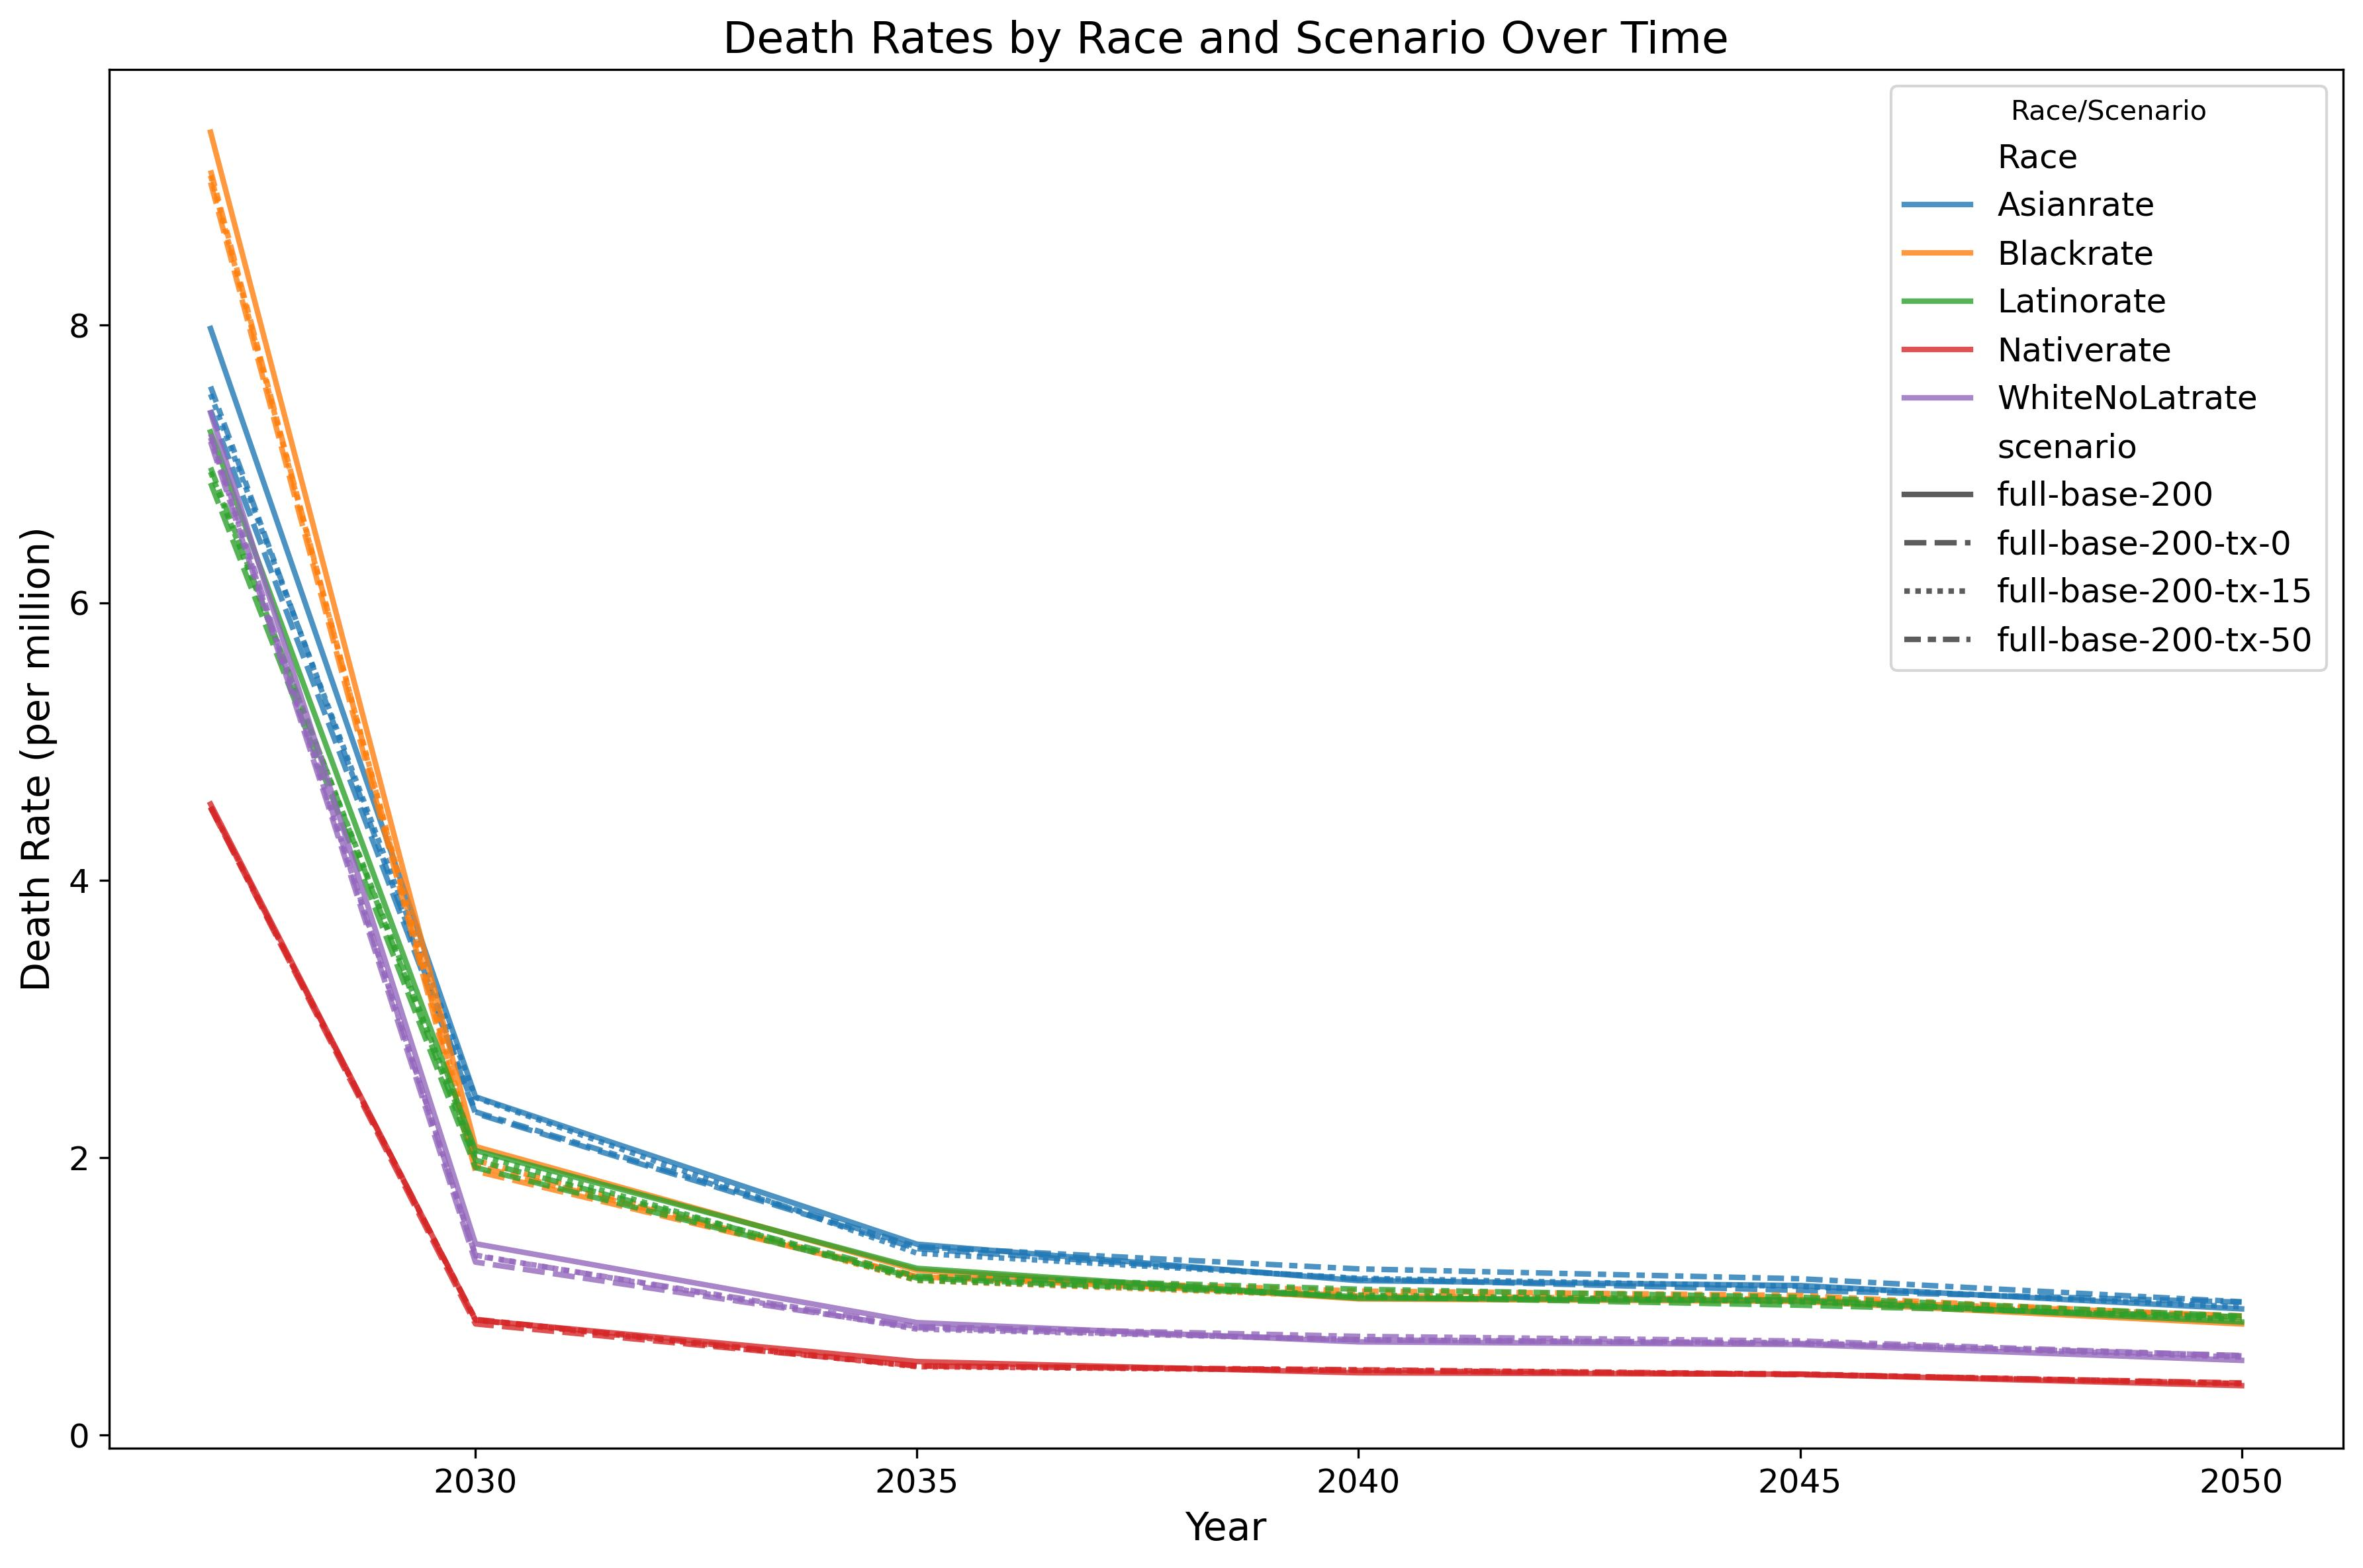
\includegraphics[width=1\linewidth]{Figures/Output/Compare_scenarios_transmissions-constraint_GenX.jpg}
    \caption{Death rates over time for transmission constraint scenarios}
    \label{TransmissionConstraint}
\end{figure}

\section{Conclusion}
This paper presents projections for how numerous different transition scenarios calculated using four different open-source models will affect the distribution of pollution exposure through 2050.  We find that pollution projections are highly synchronized across models.  Moreover, we find that a more aggressive energy transition could save more than 2,000 lives per year relative to the current policies trajectory.  All model results point towards a dramatic decrease in deaths for all racial groups.

\begin{singlespace}
\newpage
\bibliographystyle{jpe}
%\bibliographystyle{econometrica}
\bibliography{references.bib}
\end{singlespace}

\end{document}